%\documentclass[11pt]{article}
\documentclass[11pt,onecolumn]{scrartcl}
%\documentclass[11pt,onecolumn,fleqn]{scrartcl}
\usepackage[utf8]{inputenc}
\usepackage{amsmath,amssymb,amsfonts,mathrsfs,amsthm}
\usepackage[top=2cm,bottom=3cm,left=2.5cm,right=2cm]{geometry}
\usepackage{amssymb}
\usepackage{listings}
\usepackage{array}
\usepackage{mathtools}
\usepackage{dsfont}
\usepackage{graphicx}
\usepackage{pdfpages}
%\usepackage[textsize=footnotesize,color=green]{todonotes}
\usepackage{algorithm, algorithmic}
\usepackage{tikz}
\usepackage{subfigure}
%\usetikzlibrary{%
%    decorations.pathreplacing,%
%    decorations.pathmorphing%
%}
\usepackage[normalem]{ulem}

\newcommand{\bs}[1]{\boldsymbol{#1}}
\DeclareMathOperator{\diag}{diag}

\newcommand{\equaldef}{\stackrel{\mathrm{def}}{=}}

\newcommand{\tablab}[1]{\label{tab:#1}}
\newcommand{\tabref}[1]{Table~\ref{tab:#1}}

\newcommand{\theolab}[1]{\label{theo:#1}}
\newcommand{\theoref}[1]{\ref{theo:#1}}
\newcommand{\eqnlab}[1]{\label{eq:#1}}
\newcommand{\eqnref}[1]{\eqref{eq:#1}}
\newcommand{\seclab}[1]{\label{sec:#1}}
\newcommand{\secref}[1]{\ref{sec:#1}}
\newcommand{\lemlab}[1]{\label{lem:#1}}
\newcommand{\lemref}[1]{\ref{lem:#1}}

\newcommand{\mb}[1]{\mathbf{#1}}
\newcommand{\mc}[1]{\mathcal{#1}}
\newcommand{\nor}[1]{\left\| #1 \right\|}
\newcommand{\snor}[1]{\left| #1 \right|}
\newcommand{\LRp}[1]{\left( #1 \right)}
\newcommand{\LRs}[1]{\left[ #1 \right]}
\newcommand{\LRa}[1]{\left< #1 \right>}
\newcommand{\LRc}[1]{\left\{ #1 \right\}}
\newcommand{\tanbui}[2]{\textcolor{blue}{\sout{#1}} \textcolor{red}{#2}}
\newcommand{\Grad} {\ensuremath{\nabla}}
\newcommand{\Div} {\ensuremath{\nabla\cdot}}

\newcommand{\vect}[1]{\ensuremath\boldsymbol{#1}}
\newcommand{\tensor}[1]{\underline{\vect{#1}}}
\newcommand{\del}{\Delta}
\newcommand{\grad}{\nabla}
\newcommand{\curl}{\grad \times}
\renewcommand{\div}{\grad \cdot}
\newcommand{\ip}[1]{\left\langle #1 \right\rangle}
\newcommand{\eip}[1]{a\left( #1 \right)}
\newcommand{\pd}[2]{\frac{\partial#1}{\partial#2}}
\newcommand{\pdd}[2]{\frac{\partial^2#1}{\partial#2^2}}

\newcommand{\circone}{\ding{192}}
\newcommand{\circtwo}{\ding{193}}
\newcommand{\circthree}{\ding{194}}
\newcommand{\circfour}{\ding{195}}
\newcommand{\circfive}{\ding{196}}

\def\arr#1#2#3#4{\left[
\begin{array}{cc}
#1 & #2\\
#3 & #4\\
\end{array}
\right]}
\def\vecttwo#1#2{\left[
\begin{array}{c}
#1\\
#2\\
\end{array}
\right]}
\def\vectthree#1#2#3{\left[
\begin{array}{c}
#1\\
#2\\
#3\\
\end{array}
\right]}
\def\vectfour#1#2#3#4{\left[
\begin{array}{c}
#1\\
#2\\
#3\\
#4\\
\end{array}
\right]}

\newtheorem{proposition}{Proposition}
\newtheorem{corollary}{Corollary}
\newtheorem{theorem}{Theorem}
\newtheorem{lemma}{Lemma}

\newcommand{\G} {\Gamma}
\newcommand{\Gin} {\Gamma_{in}}
\newcommand{\Gout} {\Gamma_{out}}

\author{Tan Bui \and Jesse Chan \and Leszek Demkowicz \and Norbert Heuer}
\title{Robust DPG stability II}
\date{}
\begin{document}

\tableofcontents
\maketitle

\section{Introduction}

\subsection{Singular perturbation problems and robustness}

Standard Bubnov-Galerkin methods tend to perform poorly for the class of partial-differential equations known as singularly perturbed problems, where a given parameter $\epsilon$ may approach either $0$ or $\infty$ in the context of physical problems.  This poor performance is captured by the error bound
\[
\|u-u_h\|_E \leq C(\epsilon) \inf_{w_h}\|u-w_h\|_U
\]
The growth of $C$ with $\epsilon$ is referred to as a loss of robustness, where the bound on the error in the finite element solution by the best approximation error increases as $\epsilon\rightarrow 0$.  Intuitively, as our singular perturbation parameter changes, our finite element error is bounded more and more loosely by the best approximation error, allowing for degradation of the solution for very small $\epsilon$.  

A well-known example is the growth of spurious oscillations in the finite element solution of the 1D convection-diffusion problem $ u'-\epsilon u'' = f$ (with Dirichlet boundary conditions) as $\epsilon\rightarrow 0$.  Another class of examples are wave propagation problems, in which the singular perturbation parameter is the wavenumber, $k\rightarrow \infty$.  The lack of robustness in this case manifests as ``pollution" error, a phenomenon where the finite element solution degrades over many wavelengths (commonly manifesting as a phase error between the FE solution and the exact solution).  

Traditionally, instability/loss of robustness has been dealt with using residual-based stabilization.  Given some variational form, the problem is modified by adding to the bilinear form a factor of the residual, scaled by a stabilization constant $\tau$.  The most well-known example of this is the streamline-upwind Petrov-Galerkin method, which is a stabilized method for solving the convection-diffusion equation using piecewise linear continuous finite elements \cite{SUPG}.  

The addition of residual-based stabilization terms can also be interpreted as a modification of the test functions - in other words, stabilization can be achieved by changing the test space for a given problem.  This idea can be generalized under the idea of \textit{optimal test functions}.  

%\textcolor{red}{add bit about SUPG/residual-based stabilization terms and test functions}

\subsection{Optimal test functions}
The idea of optimal test functions was introduced by Demkowicz and Gopalakrishnan in \cite{DPG2}.  Conceptually, these optimal test functions are the result of a minimum residual method applied to the operator form of a variational equation.  Given Hilbert spaces $U$ and $V$ and a variational problem $b(u,v) = l(v)$, $\forall u\in U, v\in V$, we can identify $B:U\rightarrow V'$ and $l \in V'$ 
\[
\left.\begin{array}{c}
b(u_h,v) = \langle Bu_h,v\rangle  \\
l(v) = \langle l,v\rangle
\end{array}\right\}
\Longleftrightarrow Bu_h = l
\]
We seek the minimization of the residual in the dual norm
\[
\min_{u_h\in U_h} J(u_h) = \frac{1}{2}\|Bu_h-l\|_{V'}^2 = \frac{1}{2} \sup_{v\in V} \| b(u_h,v)-l(v)\|_{V}^2
\]
Recall $R_V$, the Riesz operator $\langle R_V v,\delta v\rangle = (v, \delta v)_V$ identifying elements of Hilbert space with elements of the dual.  As $R_V$ and its inverse are isometries, $\|f\|_{V'} = \|R_V^{-1} f\|_V$, and 
\[
\min_{u_h\in U_h} J(u_h) = \frac{1}{2}\|Bu_h-l\|_{V'}^2 =  \frac{1}{2}\|R_V^{-1}(Bu_h-l)\|_V^2
\]
First order optimality conditions require the Gateux derivative to be zero in all directions $u_h \in U_h$.  
\begin{align*}
\left(R_V^{-1}(Bu_h-l),R_V^{-1}B\delta u_h\right)_V &= 0, \quad \forall \delta u_h \in U_h \\
\rightarrow \langle Bu_h-l, v_h\rangle &= 0, \quad v_h = R_V^{-1}B\delta u_h
\end{align*}
which returns a standard variational equation $b(u_h,v_h) - l(v_h) = 0$, for the specific choice of test functions $v_h = R_V^{-1}B\delta u_h$.  We identify the \textit{trial-to-test} operator $T = R_V^{-1}B$, which maps a trial function $u_h$ to its corresponding \textit{optimal} test function $v_h = Tu_h$.  These test functions can be solved for by solving the auxiliary variational problem
\[
\left(v_h,\delta v\right)_V = b(u_h,\delta v)
\]

Finally, while the above variational problem is a global operation for standard continuous test spaces, the use of discontinuous test spaces reduces it to a local problem that can be solved in an element-by-element fashion.  In practice, this variational problem can rarely be solved exactly, but instead is solved approximately using the standard Bubnov-Galerkin method and an ``enriched" subspace of $V$. We assume the corresponding error in approximation of the optimal test functions is negligible for the scope of this paper.  Further work concerning the effect of approximation error in the computation of optimal test functions can be found in \cite{practicalDPG}.

Under the standard conditions for well-posedness of the continuous variational problem, the discrete DPG method delivers the best approximation error in the ``energy norm" $\|u\|_E = \sup \frac{b(u,v)}{\|v\|_V}$.  Additionally, the actual energy error $\|u-u_h\|_E$ is computable through $\|e_h\|_V$, where
\[
\left(e_h,\delta v\right)_V = b(u-u_h,v) = b(u_h,v)-l(v)
\]
This is simply a consequence of the least-squares nature of DPG; the energy error is simply the measure of the residual in the proper norm.  

\subsection{Variational form}

The DPG (discontinuous Petrov-Galerkin) method is the pairing of the concept of computable optimal test functions with the so-called ``ultra-weak formulation", where the regularity requirement on each solution variable is relaxed through integration by parts.  Moreover, to maintain conformity while seeking an $L^2$ setting on interior ``field" variables, boundary terms are identified as additional new unknowns.  The result is a hybridized DG method with locally supported optimal test functions.  For a given operator equation $Au = f$, the ultra-weak formulation is 
\[
b\left(\left(\widehat{u},u\right),v\right) - l(v) = \langle \widehat{u}, [v] \rangle - (u,A^*v) - (f,v) = 0
\]
where $A^*$ is the formal adjoint resulting from integration by parts, and $[v]$ is the jump of $v$ across element boundaries.  

\subsection{Induced norms}

Up to now, we have neglected discussion of the proper choice of inner product/norm on the space $V$.  This choice is important, as the choice of norm on $V$ determines the norm on $U$ in which DPG is optimal. Whether a particular choice of norm on $V$ norm is ``good" or not is problem-dependent; however, there is an important canonical choice of test norm for any given variational form.  

An important relationship is the duality of the energy norm and test norm; under the assumption of injectivity of the adjoint of our variational 	operator $B$, for any choice of energy norm on $U$, the test norm $\|v\|_V$ inducing it can be recovered via duality
\begin{align}
\| v \|_{V,U} = \sup_{u \in U\setminus \{0\}} \frac{b\left(u,v\right)}{\left\| u \right\|_U} \label{norm_duality}
\end{align}
If the solution is in $U$, then choosing $\|v\|=\|v\|_{V,U}$ implies $\|u\|_E = \|u\|_U$. The proof is simple; we have by definition that $b(u,v) \leq \|u\|_U\|v\|_{V,U}$. The reverse $b(u,v) \leq \|u\|_U\|v\|_{V,U}$ is proved by
\[
\inf_{u\in U} \frac{\|u\|_E}{\|u\|_U} = \inf_{u\in U} \sup_{v\in V}\frac{b(u,v)}{\|v\|_{V,U}\|u\|_U} = \inf_{v\in V} \sup_{u\in U}\frac{b(u,v)}{\|v\|_{V,U}\|u\|_U} = \inf_{v\in V} \frac{\|v\|_{V,U}}{\|v\|_{V,U}} = 1
\]
where we're able to switch the order of $\inf$ and $\sup$ due to the injectivity of $B$ (see  \cite{BabuskaEquivBrezzi}). 

As a consequence of \eqref{norm_duality}, given two norms on $U$, $\|\cdot\|_{U_1}$ and $\|\cdot\|_{U_2}$, if $\|u\|_{U_1} \leq \|u\|_{U_2}$, we have the equivalent statement
\begin{align*}
\| v \|_{V,U_1} = \sup_{u \in U\setminus \{0\}} \frac{b\left(u,v\right)}{\left\| u \right\|_{U_1}} \geq  \sup_{u \in U\setminus \{0\}} \frac{b\left(u,v\right)}{\left\| u \right\|_{U_2}} = \| v \|_{V,U_2} 
\end{align*}
In other words, showing an inequality between two norms on $U$ is equivalent to showing the reverse inequality between the respective induced norms on $V$.  

\subsection{Optimal and quasi-optimal test norms}

The duality between test norm and variational form holds for any particular variational form, though it is often difficult to determine analytically the form of $\|v\|_{V,U}$.  However, for the DPG ultra-weak formulation, there is an important test norm that results from a specific induced norm on $U$.  
Define the norm on $U$
\[
\|u\| = C_1\|u\|_{L^2} + C_2\|\widehat{u}\|
\]
where the norm on $\widehat{u}$ is taken to be the minimum energy extension norm
\[
\|\widehat{u}\| = \inf_{w\in V, \left.w\right|_{\Gamma_h}=\widehat{u}} \|w\|_V
\]
Then, the induced test norm is 
\begin{align*}
\|v\| &= \sup_{u,\widehat{u}} \frac{\langle \widehat{u}, [v] \rangle - (u,A^*v)}{C_1\|u\|_{L^2} + C_2\|\widehat{u}\|} \\
&\leq \frac{1}{C_1}\sup_{u} \frac{(u,A^*v)}{\|u\|_{L^2}} + \frac{1}{C_2}\sup_{\widehat{u}} \frac{\langle \widehat{u}, [v] \rangle}{\|\widehat{u}\|}\\
&= \frac{1}{C_1}\|A^*v\|_{L^2} + \frac{1}{C_2}\sup_{\widehat{u}} \frac{\langle \widehat{u}, [v] \rangle}{\|\widehat{u}\|}
\end{align*}
where we have used the Cauchy-Schwarz inequality, and eliminated the supremum by noting the inequality is tight.  We define $\|u\|_{\rm opt}$ as such a norm with $C_1=C_2 = 1$,
\[
\|u\|_{\rm opt} = \|u\|_{L^2} + \|\widehat{u}\|.
\]
which induces the so-called ``optimal test norm"
\[
\|v\|_{\rm opt} = \|A^*v\|_{L^2} + \left(\sup_{\widehat{u}} \frac{\langle \widehat{u}, [v] \rangle}{\|\widehat{u}\|}\right)
\]
This is, in some sense, the canonical or ideal test norm; given any well-posed variational problem, DPG under the optimal test norm will return the best finite element approximation in both field and flux variables. 

The norm $\|v\|_{\rm opt}$ is non-localizable, however - the optimal test norm is induced by a global inner product due to the presence of the jump terms.  Solving for optimal test functions under this optimal norm (through inversion of Riesz map correspdongin to this inner product) will result in expensive global problems, making this an impractical norm to work with.  

In practice, an approximation is made by removing such boundary terms and replacing them with scaled $L^2$ norms of the field variables, producing so-called \textit{quasi-optimal} test norm
\[
\|v\|_{\rm qopt} \coloneqq \|A^*v\|_{L^2} + \alpha \|v\|_{L^2}
\]
where $\alpha \in \mathbb{R}$ is chosen to complete the seminorm defined by $\|A^*v\|_{L^2}$.  This optimal test norm has been shown to induce a well-posed DPG method for any well-posed ultra-weak formulation in the context of Friedrichs' systems of equations \cite{DPGFriedrichs}.  

The DPG method is currently being analyzed for both acoustic and elastic waves in context of the Helmholtz equation and equations of linear elasticity.  Numerically, DPG appears to provide a ``pollution-free" method without phase error for these problems under the ``quasi-optimal" test norm with a specific scaling of the regularizing $L^2$ terms \cite{DPG4}. Similar results have also been obtained with the quasi-optimal test norm in the context of the elasticity \cite{DPGElas} and linear Stokes equation \cite{Camellia}. 

\section{Model problem and robustness}

We can now translate the above abstract language to a concrete model problem in computational fluid dynamics.  We consider the model convection-diffusion problem on domain $\Omega$ with boundary $\Gamma$
\begin{align}
\div (\beta u) - \epsilon\Delta v &= f  \label{primal}
\end{align}
in first order form
\begin{align*}
\div (\beta u - \sigma) &= f  \\
\frac{1}{\epsilon}\sigma - \grad u &= 0
\end{align*}
with the corresponding variational form 
\begin{align*}
b\left(\left(u,\sigma, \widehat{u}, \widehat{\sigma}_n\right), \left(\tau, v\right)\right) = \left(u,\div \tau - \beta \cdot \grad v\right) + \left(\sigma, \epsilon^{-1} \tau + \grad v\right) - \langle \left[\tau_n\right], \widehat{u} \rangle + \langle \widehat{f}_n, \left[v\right] \rangle 
\end{align*}
where $\left[ \tau_n \right]$ and $\left[ v\right]$ denote the jumps in $\tau_n$ and $v$, defined as
\begin{align*}
\left[ \tau_n \right] &= \tau^+ \cdot n^+ + \tau^-\cdot n^-\\
\left[ v\right] &= v^+{\rm sgn}(n^+) + v^-{\rm sgn}(n^-)
\end{align*}
Additionally, the inner products are taken element-wise over the finite element mesh $\Omega_h$, and the duality pairings are taken on $\Gamma_h$, the mesh ``skeleton", or union of edges of elements $K$ in $\Omega_h$.  The divergence and gradient operators are likewise understood to act element-wise. 

Define the interior skeleton $\Gamma_h^0 = \Gamma_h \setminus \Gamma$.  The functional setting is now well understood as well (see \cite{analysisDPG} for details) - $u,\sigma \in L^2(\Omega)$, $v \in H^1(\Omega_h)$, $\tau \in H({\rm div},\Omega_h)$, where $H^1(\Omega_h)$ and $H({\rm div},\Omega_h)$ are element-wise ``broken" Sobolev spaces.  By duality, $\widehat{u}$ lives in $H^{1/2}(\Gamma_h)$, the trace space of $H^1(\Omega_h)$, while $\widehat{f}_n$ comes from $H^{-1/2}(\Gamma_h)$, the normal trace space of $H({\rm div},\Omega_h)$.  

We split the boundary $\Gamma$ into three portions
\begin{align*}
\Gamma_{-} &\coloneqq \{x\in \Gamma; \beta_n(x) < 0\} \quad {\rm (inflow)}\\
\Gamma_{+} &\coloneqq \{x\in \Gamma; \beta_n(x) > 0\} \quad {\rm (outflow)}\\
\Gamma_{0} &\coloneqq \{x\in \Gamma; \beta_n(x) = 0\}
\end{align*}
We adopt a new inflow boundary condition, given by Hesthaven et al in \cite{Hesthaven96astable}, where we set
\[
\beta_n u - \sigma_n = f_n = u_0
\]
on $\Gamma_-$, and continue with the wall boundary condition $u=0$ on $\Gamma_+$.  For our model problem, as for most problems of interest in CFD, we expect $\grad u$ to be small near the inflow, and that the solutions to \eqref{primal} using $u=u_0$ and $\beta_n u - \sigma_n = f_n = u_0$ should converge to each other for sufficiently small $\epsilon$.  Under these new boundary conditions, our variational problem $b(u,v) = l(v)$ is now defined by
\begin{align*}
b\left(\left(u,\sigma, \widehat{u}, \widehat{\sigma}_n\right), \left(\tau, v\right)\right) &= \left(u,\div \tau - \beta \cdot \grad v\right) + \left(\sigma, \epsilon^{-1} \tau + \grad v\right) - \langle \left[\tau_n\right], \widehat{u} \rangle_{\Gamma_-\cup \Gamma_h^0} + \langle \widehat{f}_n, \left[v\right] \rangle_{\Gamma_+ \cup \Gamma_h^0} \\
l\left(\left(\tau,v\right)\right) &= \left(f, v\right) + \langle \left[\tau_n\right], \widehat{u} \rangle_{\Gamma_+} - \langle \widehat{f}_n, \left[v\right] \rangle_{\Gamma_-} 
\end{align*}

\subsection{Norms on $U$}

Given the boundary conditions on $\widehat{u}$ and $\widehat{f}_n$, we can now also define the trace norms as (canonical) minimum energy extension norms (taking into account the respective lifts of $\widehat{u}$ and $\widehat{f}_n$ on $\Gamma_+$ and $\Gamma_-$, respectively)
\begin{align*}
\|\widehat{u}\| &= \inf_{w\in H^1(\Omega), \left.w\right|_{\Gamma_+}=0, \left.w\right |_{\Gamma_h\setminus \Gamma_+ } = \widehat{u}} \|w\|_{H^1(\Omega)}\\
\|\widehat{f}_n\| &= \inf_{q\in H({\rm div},\Omega), \left.q\cdot n\right|_{\Gamma_-}= 0, \left. q\cdot n \right |_{\Gamma_h} = \widehat{f}_n} \|q\|_{H({\rm div},\Omega)}
\end{align*}
Additionally, throughout the rest of this work, we denote norms on $u$ and $\sigma$ as
\begin{align*}
\|u\| &= \|u\|_{L^2} \\
\|\sigma\| &= \|\sigma\|_{L^2}
\end{align*}
We will construct norms on $U$ as combinations of norms on each variable
\[
\left\|\left(u,\sigma,\widehat{u},\widehat{f}_n\right)\right\|_U = C_1 \|u\| + C_2 \|\sigma\| + C_3 \|\widehat{u}\| + C_4 \|\widehat{f}_n\|.
\]
\subsection{Norms on $V$}

%We will denote $\|\cdot \| = \|\cdot\|_{L^2}$ for all functions defined on $\Omega_h$. 
As $\tau \in H({\rm div},\Omega_h)$ and $v \in H^1(\Omega_h)$, we will construct norms on $v$ and $\tau$ using some combination of terms which are equivalent to the canonical $H^1(K) \times H({\rm div},K)$ norm over a single element
\[
\|\left(\tau,v\right)\|_{H^1(K) \times H({\rm div},K)} = \|v\|_{L^2(K)}^2 + \|\grad v\|_{L^2(K)}^2  + \|\tau\|_{L^2(K)}^2 + \|\div \tau\|_{L^2(K)}^2
\]
The squared norm over the entire triangulation $\Omega_h$ is defined to be the squared sum of contributions from each element.  The exact norms that we will place on $V$ will be determined later. 

The norms on the skeleton $\Gamma_h$ for $v$ and $\tau$ are defined by duality from the bilinear form
\begin{align*}
\|[\tau\cdot n]\| &= \|[\tau\cdot n]\|_{\Gamma_h \setminus \Gamma_+} \coloneqq \sup_{w\in H^1(\Omega), \left.w\right|_{\Gamma_+} = 0} \frac{\langle [\tau \cdot n], w\rangle}{\|w\|_{H^1(\Omega)}}\\
\|[v]\|&=\|[v]\|_{\Gamma_h^0 \cup \Gamma_+} \coloneqq \sup_{\eta\in H({\rm div};\Omega), \left.\eta\cdot n\right|_{\Gamma_- \cup \Gamma_0} = 0} \frac{\langle v, \eta\cdot n\rangle}{\|\eta\|_{H({\rm div},\Omega)}}
\end{align*}

\subsection{Approximability of the quasi-optimal test norm}%\textcolor{red}{Make new subsection on robustness here, reorganize}}

For convection-diffusion, the quasi-optimal test norm is 
\[
\|\left(\tau, v\right)\|_V^2 = \| \div \tau - \beta \cdot \grad v \|_{L^2}^2 + \| \epsilon^{-1} \tau + \grad v \|_{L^2}^2 + C_1\|v\|_{L^2} + C_2\|\tau\|_{L^2}
\]
for some choice of constants $C_1$ and $C_2$.  
%We note that the optimal test norm will automatically guarantee the robust bound $\|\left(\tau, v\right)\|_V \leq \|u\|_{L^2}$.  
However, use of this norm for the convection-diffusion problem is difficult - the variational problem for optimal test functions using the quasi-optimal test norm is equivalent to a reaction-diffusion system \cite{DBLP:journals/procedia/NiemiCC11}.  Transforming the problem to the reference element reveals that the inversion of the inner product associated with the optimal test norm will induce strong boundary layers of width $\epsilon/h^2$ in the optimal test functions.  In comparison, in Helmholtz and wave propagation problems, the mesh size tends to be on the order of the wavelength/singular perturbation parameter, resulting in smooth optimal test functions that are much easier to approximate over the reference element.  As the relevant range of $\epsilon$ for physical problems is $1e-7$, solving on partially under-resolved meshes is unavoidable, and the approximability of the optimal test functions must be addressed to take advantage of the properties of DPG.  

In the application of DPG in \cite{DPG1,DPG2,DPG3,DPG4}, the approximation of optimal test functions is done using the enriched test space $V = \cup_{K} P^{p+\Delta p}(K)$, where $p$ is the polynomial order of the trial space on a given element $K$.  In other words, optimal test functions are approximated element-by-element using polynomials whose order is $\Delta p$ more than the local order of approximation.  Under this scheme, the approximation of optimal test functions is tied to the effectiveness of the $p$-method.  Unfortunately, for problems with boundary layers (including the approximation of optimal test functions under the quasi-optimal test norm), the $p$-method performs very poorly.  

Resolving such boundary layers for an underresolved mesh has been investigated numerically using specially designed (Shishkin) subgrid meshes by Niemi, Collier, and Calo in \cite{DBLP:journals/procedia/NiemiCC11}.  However, even with Shishkin meshes, the approximation of optimal test functions under the quasi-optimal norm is difficult and far more expensive and complex to implement than approximation of test functions using a simple $p$-enriched space for $V$. We approach this from a different perspective, looking instead for robust test norms which do not induce boundary layers in the approximation of optimal test functions, and do so by formulating a general approach to analyzing the behavior of DPG under a given test norm.  

The estimates and proofs in this paper are largely based off of techniques and prior work done in \cite{DPGrobustness} and \cite{analysisDPG}; for further details, we encourage readers to consult these two publications as well.  The primary contributions in this paper are stronger stability estimates for a new inflow boundary condition and a slightly different test norm.  

\section{Strategy for proving robustness under a given test norm}

The main goal of this paper is to derive a test norm that \textit{does not induce boundary layers in the optimal test functions}, but still induces an energy norm \textit{that does not lose robustness as $\epsilon \rightarrow 0$}.  The first condition is satisfied by first decoupling norms on $\left(\tau,v\right)$ such that
\[
\left\|\left(\tau,v\right)\right\|_V = \|\tau\|_{H({\rm div},\Omega_h)} +  \|v\|_{H^1(\Omega_h)}.
\]
where $\|\tau\|_{H({\rm div},\Omega_h)}$ and $ \|v\|_{H^1(\Omega_h)}$ are both constructed as the sum of norm and seminorms on each respective space.  Ensuring that each seminorm/normed term is of the same order will allow for smooth solutions (under some assumptions on $\beta$).  The avoidance of boundary layers in the test norm will be described in more detail in the section detailing numerical experiments.  
\textcolor{red}{Why are we allowed to have $\beta\cdot \grad v$ of order 1 while we have other terms of order $O({\rm Pe})$?  Why does this term not induce boundary layers?}

Showing the second condition on robustness is equivalent to showing the robust boundedness of the energy error from above and below by norms on $U$ 
\[
\left\| \left(u,\sigma,\widehat{u},\widehat{f}_n\right)\right \|_{U,1} \lesssim  \left\| \left(u,\sigma,\widehat{u},\widehat{f}_n\right)\right \|_E \lesssim \left\| \left(u,\sigma,\widehat{u},\widehat{f}_n\right)\right \|_{U,2}
\]
where $\lesssim$ denotes a bound by a constant that will not grow as $\epsilon \rightarrow 0$.  
%$\left\| \left(u,\sigma,\widehat{u},\widehat{f}_n\right)\right \|_U \lesssim \left\| \left(u,\sigma,\widehat{u},\widehat{f}_n\right)\right \|_E$.  
Our strategy for proving such a bound is broken down into three parts.  

\subsection{Equate relations between norms on $U$ and norms on $V$}
\label{sec:strategy1}
We begin with a given norm on $U$
\[
\left\|\left(u,\sigma,\widehat{u},\widehat{f}_n\right)\right\|_U = C_1 \|u\| + C_2 \|\sigma\| + C_3 \|\widehat{u}\| + C_4 \|\widehat{f}_n\|.
\]
By \eqref{norm_duality}, the duality of test norm and energy norm, a norm of this form induces the test norm
\begin{align*}
\|\left(v,\tau\right)\|_{V,U} &= \sup_{\left(u,\sigma,\widehat{u},\widehat{f}_n\right)\in U}\frac{b\left(\left(u,\sigma,\widehat{u},\widehat{f}_n\right),\left(\tau,v\right)\right)}{C_1\|u\| + C_2\|\sigma\| + C_3\epsilon\|\widehat{u}\|+ C_4\sqrt{\epsilon}\|\widehat{u}\|}\\
&= \sup_{\left(u,\sigma,\widehat{u},\widehat{f}_n\right)\in U}\frac{\left(u,\div \tau - \beta \cdot \grad v\right) + \left(\sigma, \epsilon^{-1} \tau + \grad v\right) - \langle \left[\tau_n\right], \widehat{u} \rangle_{\Gamma_-\cup \Gamma_h^0} + \langle \widehat{f}_n, \left[v\right] \rangle_{\Gamma_+ \cup \Gamma_h^0}}{C_1\|u\| + C_2\|\sigma\| + C_3\epsilon\|\widehat{u}\|+ C_4\sqrt{\epsilon}\|\widehat{u}\|}\\
& \leq \frac{1}{C_1}\|g\| + \frac{1}{C_2}\|f\| + \frac{1}{C_3}\sup_{\widehat{u}\neq 0, \left.\widehat{u}\right|_{\Gamma_+} = 0} \frac{\langle [\tau\cdot n], \widehat{u}\rangle}{\|\widehat{u}\|} +\frac{1}{C_4}\sup_{\widehat{f}_n\neq 0, \left.\widehat{f}_n\right|_{\Gamma_-}=0}\frac{\langle \widehat{f}_n, [v]\rangle}{\|\widehat{f}\|}
\end{align*}
where $f$ and $g$ are defined as 
\begin{align*}
g &\coloneqq \div \tau - \beta \cdot \grad v\\
f &\coloneqq \epsilon^{-1}\tau + \grad v
\end{align*}
which, by definition of the boundary norms, gives the characterization of the induced test norm 
\[
\|\left(v,\tau\right)\|_{V,U} \leq \frac{1}{C_1}\|g\| + \frac{1}{C_2}\|f\| + \frac{1}{C_3}\|[\tau\cdot n]\| + \frac{1}{C_4}\|[v]\|
\]
\textcolor{red}{is this an equality? Is the inequality attainable, and thus attained in the supremum?} We can now use this relation to compare two different norms on $U$ by comparing their induced norms on $V$.  Additionally, showing a robust inequality between two norms on $U$ is similarly equivalent to showing the robust reverse inequality in the induced norms on $V$.  

\subsection{Decomposition into analyzable components}
\label{sec:strategy2}

After reducing the problem of comparing norms on $U$ to comparing norms on $V$, we break the analysis of $\left(\tau,v\right) \in V$ into the analysis of subproblems.  Define the decomposition
\[
\left(v,\tau\right) = \left(v_0,\tau_0\right) + \left(v_1,\tau_1\right) + \left(v_2,\tau_2\right),
\]
where $\left(v_1,\tau_1\right)$ satisfies 
\begin{align*}
\epsilon^{-1}\tau_1 + \grad v_1 &= 0\\
\div \tau_1 - \beta\cdot \grad v_1 &=  \div \tau - \beta\cdot \grad v = g,
\end{align*} 
Likewise, we define $\left(v_2,\tau_2\right)$ as satisfying
\begin{align*}
\epsilon^{-1}\tau_2 + \grad v_2 &= \epsilon^{-1}\tau + \grad v = f\\
\div \tau_2 - \beta\cdot \grad v_2 &= 0
\end{align*}
We will additionally require both $\left(\tau_1,v_1\right)$ and $\left(\tau_2,v_2\right)$ to come from $H({\rm div}, \Omega)\times H^1(\Omega)$, and to satisfy boundary conditions
\begin{align}
\tau_i\cdot n &= 0, \quad x \in \Gamma_- \label{bc_1}\\
v_i &= 0, \quad x \in \Gamma_+ \label{bc_2}
\end{align}
for $i = 1, 2$.  The selection of $H({\rm div}, \Omega)\times H^1(\Omega)$ conforming test functions satisfying the specific above boundary conditions removes the contribution of the jump terms over the skeleton $\Gamma_h$ in the bilinear form, allowing us to bound components of the induced test norm separately from each other.   

Finally, by construction, $\left(v_0,\tau_0\right)$ must satisfy 
\begin{align*}
\epsilon^{-1}\tau_0 + \grad v_0 &= 0\\
\div \tau_0 - \beta\cdot \grad v_0 &= 0
\end{align*}
with jumps
\begin{align*}
[v_0] &= [v], \quad x\in \Gamma_h^0\\
[\tau_0 \cdot n] &= [\tau \cdot n], \quad x\in \Gamma_h^0.
\end{align*}
By $\left(v_0,\tau_0\right) = \left(v,\tau\right) - \left(v_1,\tau_1\right) - \left(v_2,\tau_2\right)$, $\left(v_0,\tau_0\right)$ must satisfy boundary conditions
\begin{align}
v_0 &= v, \quad x\in \Gamma_+ \label{bc_1}\\
\tau_0 \cdot n &= \tau \cdot n, \quad x\in \Gamma_-\cup \Gamma_0. \label{bc_2}
\end{align}

We have now decomposed any arbitrary test function $\left(\tau,v\right)$ into a single discontinuous portion and two conforming portions.  Showing the robust bound of $\|\left(v,\tau\right)\|_V$ from above and below (by norms $\|\cdot \|_{V,1}$ and $\|\cdot \|_{V,2}$ on $V$, respectively) reduces to showing the robust bound of each component 
\[
\|\left(\tau,v\right)\|_{V,1} \lesssim \|\left(v_{0},\tau_{0}\right)\|_V, \|\left(v_{1},\tau_{1}\right)\|_V, \|\left(v_{2},\tau_{2}\right)\|_V \lesssim \|\left(\tau,v\right)\|_{V,2}
\]
Bounding $\|\left(\tau_0,v_0\right)\|$ requires the use of techniques and decompositions first developed in \cite{analysisDPG} and adapted to convection-diffusion in \cite{DPGrobustness}.  However, due to the conforming nature of $\left(\tau_1,v_1\right)$ and $\left(\tau_2,v_2\right)$, the bound from above of test functions $\|\left(v_{1},\tau_{1}\right)\|_V, \|\left(v_{2},\tau_{2}\right)\|_V \lesssim \|g\|$ is reduced to proving classical error estimates for the adjoint equations
\begin{align}
\epsilon^{-1}\tau + \grad v &= f \label{adjoint1}\\
\div \tau - \beta\cdot \grad v &=  g, \label{adjoint2}
\end{align} 
for any choice of data $f, g\in L^2({\Omega_h})$ and boundary conditions $\left.\tau\cdot n\right|_{\Gamma_-} = 0$ and $\left.v\right|_{\Gamma_+} = 0$ 

\subsection{Deriving adjoint estimates}
\label{sec:strategy3}

The final step to constructing a robust, localizable test norm on $V$ that does not generate boundary layers is to derive adjoint stability estimates on $\tau$ and $v$ in terms of localizable normed quantities.  These normed quantities will create ``building-blocks" through which we can construct test norms, where each building block will correspond roughly to the control of $\|u\|_{L^2}$, $\|\sigma\|_{L^2}$, $\|\widehat{u}\|$, or $\|\widehat{f}_n\|$.  

We introduce first the bounds derived; the proofs will be given later. For this analysis, it will be necessary to assume certain technical conditions on $\beta$.  For each proof, we require $\beta \in C^2(\bar{\Omega})$ and $\beta, \div \beta = O(1)$.  Additionally, we will assume some or all of the following assumptions hold
\begin{align}
&\curl \beta = 0, \quad 0<C \leq \left | \beta\right |^2 + \frac{1}{2}\div \beta, \quad C = O(1) \label{a_req}\\
&\grad \beta + \grad \beta ^T - \div \beta I = O(1) \label{b_req}\\
&\div \beta = 0 \label{c_req}
\end{align}
Additionally, as these results are primarily interested in stability and robustness for $\epsilon \ll 1$, we require $\epsilon$ sufficiently small in Lemma \ref{lemma_grad}.  

Under proper assumptions on $\beta$, we have the robust bounds
\begin{itemize}
\item \textbf{Lemma \ref{lemma_stream}}: For $\beta$ satisfying \eqref{a_req} and \eqref{b_req}, $f=0$ and $v \in H^1(\Omega_h)$, satisfying boundary conditions \eqref{bc_1} and \eqref{bc_2}
\begin{align*}
\|\beta \cdot \grad v \| &\lesssim \| g\| 
\end{align*}
Similarly, from $\div \tau - \beta\cdot \grad v = g$, we get $\|\div \tau\| \lesssim \|g\|$ as well.  
\item \textbf{Lemma \ref{lemma_grad}}: For $\beta$ satisfying \eqref{a_req}, and $v \in H^1(\Omega_h)$ satisfying boundary conditions \eqref{bc_1} and \eqref{bc_2}, and for sufficiently small $\epsilon$
\begin{align*}
\epsilon \|\grad v\|^2 + \|v\|^2 &\lesssim \|g\|^2 + \epsilon \| f\|^2
\end{align*}
\item \textbf{Lemma \ref{lemma_boundary}}: For $\beta$ satisfying \eqref{a_req}, \eqref{c_req}, and $f=g=0$, 
\begin{align*}
\|\grad v\| = \frac{1}{\epsilon}\|\tau\| &\lesssim \frac{1}{\epsilon} \| [\tau\cdot n]\|_{\Gamma_h \setminus \Gamma_+} + \frac{1}{\sqrt{\epsilon}} \| [v]\|_{\Gamma_h^0 \cup \Gamma_+}
\end{align*}
\end{itemize}
Together, these estimates will be sufficient to construct a norm on $V$ and demonstrate bounds on induced test norms for different scalings of norms on $U$.  

\section{Relations between energy and $U$ norms}
\label{sec:main_bounds}
The primary result of this paper is that, if $\beta$ satisfies \ref{a_req},\ref{b_req}, and \ref{c_req}, the DPG method provides robust control over the $L^2$ error in $u$ and $\sigma$
\[
\left\|\left(u,\sigma,\widehat{u},\widehat{f}_n\right)-\left(u_h,\sigma_h,\widehat{u}_h,\widehat{f}_{n,h}\right)\right\|_{U_1} \lesssim \inf_{w\in U_h}\left\|\left(u,\sigma,\widehat{u},\widehat{f}_n\right)-w_h \right\|_{E}
\]
using the test norm
\[
\|\left(\tau, v\right)\|_{V}^2 = \|v\|^2 + \epsilon \|\grad v\|^2 + \|\beta \cdot \grad v\|^2 + \| \div \tau\|^2 + \frac{1}{\epsilon}\|\tau\|^2
\]
where $\|\cdot \|_{U_1}$ is defined as
\[
\left\|\left(u,\sigma,\widehat{u},\widehat{f}_n\right)\right\|_{U_1} \coloneqq \|u\| + \|\sigma\| + \epsilon\|\widehat{u}\|+\sqrt{\epsilon} \|\widehat{f}_n\|.
\]
%\textcolor{red}{should be explained here}. 

A second, weaker result is an upper bound on the energy norm
\[
\left\|\left(u,\sigma,\widehat{u},\widehat{f}_n\right)-\left(u_h,\sigma_h,\widehat{u}_h,\widehat{f}_{n,h}\right)\right\|_{E} \lesssim \inf_{w\in U_h}\left\|\left(u,\sigma,\widehat{u},\widehat{f}_n\right)-w_h\right\|_{U_2}
\]
where $\|\cdot \|_{U_2}$ is defined as
\[
\left\|\left(u,\sigma,\widehat{u},\widehat{f}_n\right)\right\|_{U_2}^2 \coloneqq \|u\|^2 + \frac{1}{\sqrt{\epsilon}}\left(\|\sigma\|^2 + \|\widehat{u}\|^2+ \|\widehat{f}_n\|^2\right).
\]
While the upper bound is robust, we have derived such a bound only by explicitly accounting for a factor of $\epsilon^{-1/2}$ in the bounding norm $\|\cdot \|_{U_2}$.  This implying that for very small $\epsilon$, the $L^2$ error may be much smaller than the energy error.  However, \textcolor{red}{explain why this is OK practically.}
Additionally, numerical experiments demonstrate much better results, and suggest that, at least for our examples, $\|u-u_h\|_E \sim \|u-u_h\|_{U}$, implying that the induced energy norm is equivalent to a norm on the group variable $\left(u,\sigma,\widehat{u},\widehat{f}_n\right)$ that does not grow with $\epsilon$.  

\subsection{Bound from below}

We begin by using the strategy outlined in sections~\ref{sec:strategy1}, ~\ref{sec:strategy2}, and ~\ref{sec:strategy3} to prove the robust bound of the $L^2$ error in the field variables by the energy error.  

As a consequence of \eqref{norm_duality}, assume an energy norm $\left\| u \right\|_{E,1}$ is induced by a given test norm $\| v  \|_{V,1}$.  To bound $\|\cdot\|_E$ robustly from above or below by a given norm $\left\| u \right\|_{U,2}$ on $U$ now only requires the robust bound in the opposite direction of $\| v \|_{V,1}$ by $\|v\|_{V,2}$. 

\begin{lemma}
\label{bound_from_below}
(Bound from below) If $\beta$ satisfies \eqref{a_req} and \eqref{b_req}, then for $\left(u,\sigma,\widehat{u},\widehat{f}_n\right) \in U$,
\[
\|u\| + \|\sigma\| + \epsilon\|\widehat{u}\|+ \sqrt{\epsilon}\|\widehat{u}\| \lesssim \left\|\left(u,\sigma,\widehat{u},\widehat{f}_n\right)\right\|_E
%\|u\| + \frac{1}{\sqrt{\epsilon}}\|\sigma\| + \epsilon\|\widehat{u}\|+ \sqrt{\epsilon}\|\widehat{u}\| \lesssim \left\|\left(u,\sigma,\widehat{u},\widehat{f}_n\right)\right\|_E
\]
\end{lemma}
\begin{proof}
By \eqref{norm_duality}, for 
\begin{align*}
f &= \epsilon^{-1}\tau + \grad v  \\
g &=\div \tau - \beta\cdot \grad v,
\end{align*} 
we can characterize the test norm for $\left\|\left(u,\sigma,\widehat{u},\widehat{f}_n\right)\right\|_U = C_1\|u\| + C_2\|\sigma\| + C_3\|\widehat{u}\|+ C_4\|\widehat{u}\|$ as
\begin{align*}
\|\left(v,\tau\right)\|_V &\lesssim \frac{b\left(\left(u,\sigma,\widehat{u},\widehat{f}_n\right),\left(\tau,v\right)\right)}{C_1\|u\| + C_2\|\sigma\| + C_3\|\widehat{u}\|+ C_4\|\widehat{u}\|}\\
& \simeq \frac{1}{C_1}\|g\| + \frac{1}{C_2}\|f\| + \frac{1}{C_3}\sup_{\widehat{u}\neq 0, \left.\widehat{u}\right|_{\Gamma_+} = 0} \frac{\langle [\tau\cdot n], \widehat{u}\rangle}{\|\widehat{u}\|} + \frac{1}{C_4}\sup_{\widehat{f}_n\neq 0, \left.\widehat{f}_n\right|_{\Gamma_-}=0}\frac{\langle \widehat{f}_n, [v]\rangle}{\|\widehat{f}\|},
\end{align*}
which, by definition of the boundary norms, is 
\[
\|\left(v,\tau\right)\|_V \lesssim \frac{1}{C_1}\|g\| + \frac{1}{C_2}\|f\| + \frac{1}{C_3}\|[\tau\cdot n]\| + \frac{1}{C_4}\|[v]\|
\]
We will bound $\|\left(v,\tau\right)\|_V$ for all $\left(v,\tau\right)$ satisfying \eqref{adjoint} by decomposing $\left(v,\tau\right) = \left(v_0,\tau_0\right) + \left(v_1,\tau_1\right) + \left(v_2,\tau_2\right)$ as described in section~\ref{sec:strategy2}.  
%where $\left(v_1,\tau_1\right)$ satisfies our adjoint equation \eqref{adjoint} with boundary conditions \eqref{bc_1} and \eqref{bc_2} and 
%\begin{align*}
%f &= 0\\
%g&= \div \tau - \beta\cdot \grad v,
%\end{align*} 
%and $\left(v_2,\tau_2\right)$ satisfies \eqref{adjoint} with boundary conditions \eqref{bc_1} and \eqref{bc_2} and 
%\begin{align*}
%g &= 0\\
%f &= \epsilon^{-1}\tau + \grad v.
%\end{align*}
%We note that, if $v_2$ satisfies $n\cdot \grad v_2 = n\cdot f$, by definition of $f$ and $v_2$,
%\begin{align*}
%\tau_2 \cdot n &= \epsilon n\cdot f - \epsilon n\cdot \grad v_2 = 0, \quad x\in \Gamma_- \cup \Gamma_0
%\end{align*}
%By construction, $\left(v_0,\tau_0\right)$ satisfies adjoint equations \eqref{adjoint1} and \eqref{adjoint2} with $f=g=0$, with jumps
%\begin{align*}
%[v_0] &= [v], \quad x\in \Gamma_h^0\\
%[\tau_0 \cdot n] &= [\tau \cdot n], \quad x\in \Gamma_h^0.
%\end{align*}
%By $\left(v_0,\tau_0\right) = \left(v,\tau\right) - \left(v_1,\tau_1\right) - \left(v_2,\tau_2\right)$, $\left(v_0,\tau_0\right)$ must satisfy boundary conditions
%\begin{align*}
%v_0 &= v, \quad x\in \Gamma_+\\
%\tau_0 \cdot n &= \tau \cdot n, \quad x\in \Gamma_-\cup \Gamma_0.
%\end{align*}
Robustly bounding $\|\left(v,\tau\right)\|_V$ from above reduces to robustly bounding each component 
\[
\|\left(v_{0},\tau_{0}\right)\|_V, \|\left(v_{1},\tau_{1}\right)\|_V, \|\left(v_{2},\tau_{2}\right)\|_V \lesssim \frac{1}{C_1}\|g\| + \frac{1}{C_2}\|f\| + \frac{1}{C_3}\|[\tau\cdot n]\| + \frac{1}{C_4}\|[v]\|
\]
%\begin{align*}
%\|\left(\tau, v\right)\|_{V}^2 &= \|v\|^2 + \epsilon \|\grad v\|^2 + \|\beta \cdot \grad v\|^2 + \| \div \tau\|^2 + \frac{1}{\epsilon}\|\tau\|^2 \\
%& \lesssim \|g\| + \|f\| + \epsilon^{-1}\|[\tau\cdot n]\| + \epsilon^{-1/2}\|[v]\|
%\end{align*}
\begin{itemize}
\item \textbf{Bound on $\|\left(v_{0},\tau_{0}\right)\|_V$}
 
Lemma \ref{lemma_boundary} gives control over $\epsilon\|\grad v_0\| + \frac{1}{\epsilon}\|\tau_0\|$ through
\[
\|\grad v_0\| = \frac{1}{\epsilon}\|\tau_0\| \lesssim \frac{1}{\epsilon} \| [\tau_0\cdot n]\|_{\Gamma_h \setminus \Gamma_+} + \frac{1}{\sqrt{\epsilon}} \| [v_0]\|_{\Gamma_h^0 \cup \Gamma_+} = \frac{1}{\epsilon} \| [\tau\cdot n]\|_{\Gamma_h \setminus \Gamma_+} + \frac{1}{\sqrt{\epsilon}} \| [v]\|_{\Gamma_h^0 \cup \Gamma_+}
\]
Lemma 4.2 of \cite{analysisDPG} gives us the Poincare inequality for discontinuous functions
\[
\|v_0\| \lesssim \|\grad v_0\| + \|[v]\|
\]
%Since $f=0$, by Lemma 2, $\|\beta\cdot \grad v_0\|  \lesssim \|g\| = 0$.  
Since $g = 0$, $\| \div \tau_0\| = \|\beta\cdot \grad v_0\|\lesssim \|\grad v_0\|$, which we now have control over as well.  

\item \textbf{Bound on $\|\left(v_{1},\tau_{1}\right)\|_V$}

%Given $\tau_1 \in H({\rm div};\Omega)$, $v\in H^1(\Omega)$, with boundary conditions \eqref{bc_1} and \eqref{bc_2}, $\frac{1}{\epsilon} \| [\tau_0\cdot n]\|_{\Gamma_h \setminus \Gamma_+} + \frac{1}{\sqrt{\epsilon}} \| [v_0]\|_{\Gamma_h^0 \cup \Gamma_+}=0$.
With $f = 0$, Lemma \ref{lemma_grad} provides the bound
\[
\|\beta \cdot \grad v_1 \| \lesssim \| g\|
\]
Noting that $\div \tau_1 = g+\beta\cdot \grad v_1$ gives $\|\div \tau_1 \| \lesssim \|g\|$ as well.  Lemma \ref{lemma_grad} gives
\[
\epsilon \|\grad v_1\|^2 + \|v_1\|^2 \lesssim \|g\|^2
\]
and noting that $\epsilon^{-1/2}\tau_1 = \epsilon^{1/2}v_1$ gives $\epsilon\|\grad v_1\|^2 = \epsilon^{-1}\|\tau_1\|^2 \lesssim \|g\|^2$ as well.

\item \textbf{Bound on $\|\left(v_{2},\tau_{2}\right)\|_V$}

Lemma \ref{lemma_grad} provides
\[
\epsilon \|\grad v\|^2 + \|v\|^2 \lesssim  \epsilon \| f\|^2 \leq \|f\|^2
\]
We have $\epsilon^{-1}\tau = f - \grad v$, so $\epsilon^{-1} \|\tau\| \lesssim \|f\| + \|\grad v\|$. Lemma~\ref{lemma_grad} implies $\|\grad v\|^2  \lesssim  \| f\|^2$, so for $\epsilon \leq 1$, we control $\epsilon^{-1/2}\|\tau\| \leq \epsilon^{-1}\|\tau\| \lesssim \|f\|$.  The remaining terms can be bounded by noting that, with $g = 0$, $\|\div \tau_2\| = \|\beta\cdot \grad v_2\| \lesssim \|\grad v_2\| \lesssim \|f\| $.
\end{itemize}

With these characterizations, we can conclude that $C_1 = C_2 = 1$, $C_3 = \epsilon$, and $C_4 = \epsilon^{1/2}$.  
\end{proof}

\subsection{Bound from above}

We have shown the robust bound of a norm on $U$ by energy error; for a full equivalence statement, we require a bound on the energy norm by some norm on $U$.  By the duality of the energy and test norm, this is equivalent to bounding the test norm from below, using the test norm induced by the norm on $U$ bounding the energy norm.  
\begin{lemma}

(Bound from above) For $\left(u,\sigma,\widehat{u},\widehat{f}_n\right) \in U$,
\[
\left\|\left(u,\sigma,\widehat{u},\widehat{f}_n\right)\right\|_E \lesssim \|u\| + \frac{1}{\sqrt{\epsilon}}\left(\|\sigma\| + \|\widehat{u}\|+ \|\widehat{u}\|\right)
\]

\end{lemma}
\begin{proof}
For any norm on $U$ of the form
\[
\left\|\left(u,\sigma,\widehat{u},\widehat{f}_n\right)\right\|_{U,*} = \|u\| + C_2 \|\sigma\| + C_3 \|\widehat{u}\| + C_4 \|\widehat{f}_n\|,
\]
the induced test norm is  
\begin{align*}
\| \left(\tau,v\right) \|_{V,*} &= \sup_{\left(u,\sigma,\widehat{u},\widehat{f}_n\right) \in U\setminus \{0\}} \frac{b\left(\left(u,\sigma,\widehat{u},\widehat{f}_n\right),\left(\tau,v\right)\right)}{\left\|\left(u,\sigma,\widehat{u},\widehat{f}_n\right)\right\|_E} \\
& = \sup_{\left(u,\sigma,\widehat{u},\widehat{f}_n\right) \in U\setminus \{0\}} \frac{\left(u,\div \tau - \beta \cdot \grad v\right) + \left(\sigma, \epsilon^{-1} \tau + \grad v\right) - \langle \left[\tau_n\right], \widehat{u} \rangle + \langle \widehat{f}_n, \left[v\right] \rangle
}{\|u\| + C_2 \|\sigma\| + C_3 \|\widehat{u}\| + C_4 \|\widehat{f}_n\|} \\
&\lesssim \|g\| + \frac{1}{C_2}\|f\| + \sup_{\widehat{u},\widehat{f}_n \neq 0}\frac{\langle \left[\tau_n\right], \widehat{u} \rangle + \langle \widehat{f}_n, \left[v\right] \rangle}{C_3\|\widehat{u}\| + C_4\|\widehat{f}_n\|}
\end{align*}
where $f$ and $g$ are again the loads of the adjoint problem \eqref{adjoint}.  By the triangle inequality, we have the bounds
\begin{align*}
\epsilon \|f \|^2 &\leq \epsilon^{-1} \| \tau\|^2 + {\epsilon} \|\grad v\|^2 \lesssim \| \left(\tau,v\right)\|_V^2\\
\|g \| &\leq \|\div \tau\| +  \|\beta \cdot \grad v\| \lesssim \| \left(\tau,v\right)\|_V
\end{align*}
We estimate the supremum by following \cite{DPGrobustness}; we begin by choosing $\eta \in H({\rm div}; \Omega)$, $w\in H^1(\Omega)$, such that $\left.\left(\eta-\beta w \right)\cdot n\right |_{\Gamma_+} = 0$ and $\left.w\right |_{\Gamma_-\cup\Gamma_0} = 0$, and integrating the boundary pairing by parts to get
\begin{align*}
\langle [\tau\cdot n],w\rangle + \langle [v],\left(\eta - \beta w\right)\cdot n\rangle &\lesssim \|\left(\tau,v\right)\|_V\frac{1}{\sqrt{\epsilon}}\left(\|\eta\| + \|w\|\right)\\
%\langle [\tau\cdot n],w\rangle + \langle [v],\left(\eta - \beta w\right)\cdot n\rangle 
&\lesssim \|\left(\tau,v\right)\|_V\frac{1}{\sqrt{\epsilon}}\left(\|\eta-\beta w\| + \|w\|\right)
\end{align*}
since $\|\eta\| = \|\eta - \beta w + \beta w\| \leq \|\eta - \beta w\| + \|\beta w\| \lesssim \|\eta-\beta w\| + \|w\|$.  Dividing through and taking the supremum gives
\[
\sup_{w,\eta \neq 0} \frac{\langle[\tau\cdot n],w\rangle + \langle [v],\left(\eta - \beta w\right)\cdot n\rangle}{\left(\|\eta-\beta w\| + \|w\|\right)} \lesssim \|\left(\tau,v\right)\|_V\frac{1}{\sqrt{\epsilon}}
\]
To finish the proof, define $\rho \in H^{1/2}(\Gamma_h)$ and $\phi \in H^{-1/2}(\Gamma_h)$ such that $\rho = \left.w\right|_{\Gamma_h}$ and $\phi = \left.(\eta-\beta w)\cdot n\right|_{\Gamma_h}$, and note that
\begin{align*}
\sup_{\rho,\phi \neq 0} \frac{\langle [\tau\cdot n],\rho\rangle + \langle [v],\phi \rangle}{\|\rho\|+\|\phi\|} &= \sup_{w,\eta \neq 0} \frac{\langle [\tau\cdot n],w\rangle + \langle [v],\left(\eta - \beta w\right)\cdot n\rangle}{ \|w\|+\|\eta-\beta w\|} 
\end{align*}

Together, the bounds on $\|g\|$ and $\|f\|$ imply $\left\|\left(u,\sigma,\widehat{u},\widehat{f}_n\right)\right\|_{E} \lesssim \left\|\left(u,\sigma,\widehat{u},\widehat{f}_n\right)\right\|_{U,*}$ for $C_2 = C_3 = C_4 = \frac{1}{\sqrt{\epsilon}}$.  
\end{proof}

%In \cite{DPGrobustness}, the quasi-optimal test norm was shown to induce an energy norm that is bounded from both above and below by norms on $U$ that do not grow in magnitude with $\epsilon^{-1}$.  

\section{Proof of lemmas/stability of the adjoint problem}

We reduce the adjoint problem to the scalar second order equation
\begin{equation}
- \epsilon \Delta v - \beta \cdot \grad v = g - \epsilon \div f \label{adjoint}
\end{equation}
with boundary conditions
\begin{align}
%\tau \cdot n = 
- \epsilon \grad v \cdot n &=f\cdot n, \quad x\in \Gamma_- \label{reducedbc_1}\\ 
v &= 0, \quad x\in \Gamma_+ \label{reducedbc_2}
\end{align}
and treat the cases $f=0$, $g=0$ separately.  The above boundary conditions are the reduced form of boundary conditions \eqref{bc_1} and \eqref{bc_2}. 

Additionally, the $\div$ operator is understood now in the weak sense, as the dual operator of $-\grad : H_0^1(\Omega) \rightarrow L^2(\Omega)$, such that $\div f \in \left(H_0^1(\Omega)\right)'$. The normal trace $f\cdot n$ is understood as a limit; smooth functions are dense in $H^1(\Omega)$, and we define $f\cdot n$ as the limit of $f_i\cdot n$, where $f_i \in C^\infty(\Omega)$, $f_i \rightarrow f$.
\textcolor{red}{clearly define what we mean here with the density argument}

Lemma \ref{lemma_grad} concerns the robust control of $u$ by the energy error; Lemmas \ref{lemma_stream} and \ref{lemma_boundary} concern the robust control of field variable $\sigma$ and flux/trace variables, respectively.  

\begin{lemma} 
\label{lemma_stream}
Assume $v$ satisfies \eqref{adjoint}, with boundary conditions \eqref{bc_1}, and \eqref{bc_2}, and $\beta$ satisfies \eqref{a_req} and \eqref{b_req}.  If $\div f = 0$ and $\epsilon$ is sufficiently small, 
\[
\|\beta \cdot \grad v \| \lesssim \| g\|
\]
\end{lemma}

\begin{proof}
Define $v_\beta = \beta\cdot \grad v$.  Multiplying the adjoint equation \eqref{adjoint} by $v_\beta$ and integrating over $\Omega$ gives
\[
\|v_\beta\|^2 = -\int_\Omega g v_\beta - \epsilon \int_\Omega \Delta v v_\beta
\]
Note that 
\[
-\int_{\Omega} \beta\cdot \grad v \del v = -\int_{\Omega} \beta\cdot \grad v \div \grad v
\]
Integrating this by parts, we get
\[
-\int_{\Omega} \beta\cdot \grad v \div \grad v = \int_{\Omega}\grad (\beta\cdot \grad v) \cdot \grad v  - \int_{\Gamma}n\cdot \grad v \beta\cdot\grad v
\]
Note that 
\[
\grad (\beta \cdot \grad v) = \grad \beta \cdot \grad v + \beta \cdot \grad \grad v
\]
where $\grad \beta$ and $\grad \grad v$ are understood to be tensors. Then, 
\[
\int_{\Omega}\grad (\beta\cdot \grad v) \cdot \grad v = \int_{\Omega}(\grad \beta\cdot \grad v) \cdot \grad v + \int_{\Omega}\beta\cdot \grad\grad v \cdot \grad v 
\]
Noting that $\grad v \cdot \grad \grad v = \grad\frac{1}{2}\left(\grad v\cdot \grad v\right)$, if we integrate by parts again, we get
%\[
%\int_{\Omega}\beta\cdot \grad\grad v \cdot \grad v = \frac{1}{2}\int_{\Omega}\beta\cdot \grad(\grad v \cdot \grad v ) = \frac{1}{2}\int_{\Gamma}\beta_n (\grad v \cdot \grad v ) - \frac{1}{2}\int_{\Omega}\div \beta (\grad v \cdot \grad v )
%\]
%Then, we can combine these terms to get
\begin{align*}
-\int_{\Omega}  \del vv_\beta &= - \int_{\Gamma}n\cdot \grad v \beta\cdot\grad v + \frac{1}{2}\int_{\Gamma}\beta_n (\grad v \cdot \grad v ) - \frac{1}{2}\int_{\Omega}\div \beta (\grad v \cdot \grad v ) + \int_{\Omega}(\grad \beta\cdot \grad v) \cdot \grad v\\
&= - \int_{\Gamma}n\cdot \grad v \beta\cdot\grad v + \frac{1}{2}\int_{\Gamma}\beta_n (\grad v \cdot \grad v ) + \int_{\Omega} \grad v \left(\grad \beta - \frac{1}{2}\div \beta I\right)\grad v
\end{align*}
Finally, substituting this into our adjoint equation multiplied by $v_\beta$, we get
\[
\| v_\beta\|^2 = -\int_{\Omega}g\beta\cdot \grad v +  \epsilon\int_{\Gamma}  \left( -n\cdot \grad v \beta + \frac{1}{2}\beta_n \grad v \right) \cdot \grad v + \epsilon\int_{\Omega} \grad v \left(\grad \beta - \frac{1}{2}\div \beta I\right)\grad v
\]
%The first term on the RHS can be controlled using Young's inequality. 
The last term can be bounded by our assumption on $\|\grad \beta - \frac{1}{2}\div \beta I\|^2 \leq C$.
\[
\epsilon \int_{\Omega} \grad v \left(\grad \beta - \frac{1}{2}\div \beta I\right)\grad v \leq C\frac{\epsilon}{2} \|\grad v\|^2
\]
For the boundary terms, on $\Gamma_-$, $\grad v\cdot n = 0$, reducing the integrand over the boundary to $\beta_n|\grad v|^2 \leq 0$.  On $\Gamma_+$, $v=0$ implies $\grad v \cdot \tau = 0$, where $\tau$ is a tangential direction.  An orthogonal decomposition yields $\grad v = (\grad v \cdot n) n$, reducing the above to 
\[
 \epsilon\int_{\Gamma}  -\frac{1}{2}|\beta_n| (\grad v \cdot n)^2 \leq 0
\]
leaving us with the estimate
\[
\|v_\beta\|^2 \leq  -\int_{\Omega}g\beta\cdot \grad v + C\frac{\epsilon}{2} \|\grad v\|^2
\]
Since $C=O(1)$, an application of Young's inequality and Lemma \ref{lemma_grad} complete the estimate.
\end{proof}

\begin{lemma} 
\label{lemma_grad}
Assume \eqref{a_req} holds.  Then, for $v$ satisfying equation \eqref{adjoint} with boundary conditions \eqref{bc_1}, \eqref{bc_2} and sufficiently small $\epsilon$, 
\[
\epsilon \|\grad v\|^2 + \|v\|^2 \lesssim \|g\|^2 + \epsilon \| f\|^2
\]
\end{lemma}

\begin{proof}
Since $\curl \beta=0$, and $\Omega$ is simply connected, there exists a scalar potential $\psi$, $\grad \psi = \beta$ such that $e^\psi = O(1)$.  Take the transformed function $w = e^\psi v$; following (2.26) in \cite{DPGrobustness}, we substitute $w$ into the the left hand side of equation \eqref{adjoint}, arriving at the relation  
\[
-\epsilon \Delta w - (1-2\epsilon) \beta \cdot \grad w + \left((1-\epsilon)|\beta|^2 + \epsilon \div \beta\right) w = e^\psi (g-\epsilon \div f)
\]
Multiplying by $w$ and integrating over $\Omega$ gives
\[
-\epsilon \int_\Omega \Delta ww - (1-2\epsilon) \int_\Omega\beta \cdot \grad w w + \int_\Omega\left((1-\epsilon)|\beta|^2 + \epsilon \div \beta\right) w^2 = \int_\Omega e^\psi (g-\epsilon \div f) w
\]
Integrating by parts gives
\[
-\epsilon \int_\Omega \Delta ww - (1-2\epsilon) \int_\Omega\beta \cdot \grad w w = \epsilon \left( \int_\Omega |\grad w|^2- \int_{\Gamma} w \grad w \cdot n  \right) + \frac{(1-2\epsilon) }{2} \left(\int_\Omega \div \beta w^2 - \int_\Gamma\beta_n w^2 \right)
\]
Noting that $w=0$ on $\Gamma_+$ reduces the boundary integrals over $\Gamma$ to just the inflow $\Gamma_-$.  Furthermore, we have the relation $\grad w = e^\psi(\grad v + \beta v)$.  Applying the above and boundary conditions on $\Gamma_-$, the first boundary integral becomes
\[
\int_{\Gamma_-} w \grad w \cdot n = \int_{\Gamma_-} we^\psi(\grad v + \beta v)\cdot n =  \int_{\Gamma_-} we^\psi(f\cdot n + \beta_n v)
\]
Noting $\int_{\Gamma_-}\beta_n w^2 \leq 0$ through $\beta_n<0$ on the inflow gives
\[
\epsilon \int_\Omega |\grad w|^2 + \int_\Omega \left((1-\epsilon)|\beta|^2 + \frac{1}{2} \div \beta \right) w^2 - \epsilon \int_{\Gamma_-} we^\psi f\cdot n \leq \int_\Omega e^\psi (g-\epsilon \div f) w
\]
assuming $\epsilon$ is sufficiently small.  Our assumptions on $\beta$ implies $\left((1-\epsilon)|\beta|^2 + \frac{1}{2} \div \beta \right) \lesssim 1$ and $e^\psi = O(1)$. We can then bound from below
\[
\epsilon \|\grad w\|^2 + \|w\|^2 - \epsilon \int_{\Gamma_-} we^\psi f\cdot n  \lesssim \epsilon \int_\Omega |\grad w|^2 + \int_\Omega \left((1-\epsilon)|\beta|^2 + \frac{1}{2} \div \beta \right) w^2 - \epsilon \int_{\Gamma_-} we^\psi f\cdot n 
\]
Interpreting $\div f$ as a functional, the right hand gives
\begin{align*}
\int_\Omega e^\psi (g-\epsilon \div f) w &= \int_\Omega e^\psi g + \int_\Omega \epsilon f \cdot \grad (e^\psi w) - \int_\Gamma \epsilon f\cdot n e^\psi w
\end{align*}
The boundary integral on $\Gamma$ reduces to $\Gamma_-$, which is then nullified by the same term on the left hand side, leaving us with 
\[
\epsilon \|\grad w\|^2 + \|w\|^2 \lesssim \int_\Omega e^\psi g + \int_\Omega \epsilon f \cdot \grad (e^\psi w) = \int_\Omega e^\psi g + \int_\Omega \epsilon f \cdot (\beta w + \grad w)
\]
From here, the proof is identical to \cite{DPGrobustness}; an application of Peter-Paul Young's inequality to the right hand side and bounds on $\|v\|, \|\grad v\|$ by $\|w\|,\|\grad w\|$ complete the estimate.  
%ISSUE: REMOVE BOUNDARY TERM
\end{proof}

\begin{lemma}
\label{lemma_boundary}
Let $\beta$ satisfy \eqref{a_req} and \eqref{c_req}, and let $v$ satisfy \eqref{adjoint} with $f=g=0$, and arbitrary boundary conditions.  Then, there holds
\[
\|\grad v\| = \frac{1}{\epsilon}\|\tau\| \lesssim \frac{1}{\epsilon} \| [\tau\cdot n]\|_{\Gamma_h \setminus \Gamma_+} + \frac{1}{\sqrt{\epsilon}} \| [v]\|_{\Gamma_h^0 \cup \Gamma_+}
\]
\end{lemma}
\begin{proof}
We follow \cite{analysisDPG} and \cite{DPGrobustness} in decomposing $\tau$ into $z\in H({\rm curl},\Omega)$ and $\psi\in H^1(\Omega)$ such that
\[
\tau = \left(\epsilon \grad \psi - \beta \psi\right) + \curl z
\]
Specifically, $\psi$ is chosen as the solution to 
\begin{align*}
-\epsilon \Delta \psi + \div \left(\beta \psi\right) &= -\div \tau \\
\epsilon \grad \psi \cdot n - \beta_n \psi - \tau\cdot n &= 0, \quad x\in \Gamma_-\\
\psi &= 0, \quad x\in \Gamma_+ 
\end{align*}
Since $\div \beta = 0$, we satisfy \eqref{a_req}, and can use Lemma \ref{lemma_grad} (with $f = \frac{1}{\epsilon}\tau$) to bound
\[
\epsilon \|\grad \psi\|^2 + \|\psi \|^2 = \frac{1}{\epsilon}\|\tau\|^2
\]
By the above bound and triangle inequality, 
\[
\|\curl z \| \leq \epsilon \|\grad \psi\| + \|\beta \psi\| + \|\tau\| \lesssim \frac{1}{\sqrt{\epsilon}}\|\tau\|
\]
On the other hand, using the decomposition and boundary conditions directly, we can integrate by parts to arrive at
\begin{align*}
\|\tau\|^2 &= (\tau, \epsilon \grad \psi - \beta \psi + \curl z) = (\tau, \epsilon \grad \psi) - (\tau,\beta \psi) + (\tau,\curl z)  \\
&=(\tau, \epsilon \grad \psi) + \epsilon(\grad v,\beta \psi) - \epsilon(\grad v,\curl z)  \\
&=\epsilon \langle [\tau \cdot n],\psi \rangle - \epsilon  \langle n\cdot \curl z, [v]\rangle = \epsilon \langle [\tau \cdot n],\psi \rangle_{\Gamma_h \setminus \Gamma_+} - \epsilon  \langle n\cdot \curl z, [v]\rangle_{\Gamma_h \cup \Gamma_+}\\
&\lesssim \epsilon \|[\tau \cdot n]\| \|\psi\| + \epsilon \| [v]\|\| n\cdot \curl z \| 
\end{align*}
by definition of the boundary norms on $[\tau\cdot n]$ and $[v]$.  

Applying the above estimates for $\|\psi\|$ and $\|n\cdot \curl z\|$ and noting that $\|\grad v\| = \frac{1}{\epsilon}\|\tau\|$ completes the proof.
\end{proof}

\subsection{Comparison of boundary conditions}

It's worth addressing the effect of boundary conditions on stability.  Specifically, a test norm that provides stability for one set of boundary conditions may perform poorly for another set.  Take, for example, the test norm defined in Section~\ref{sec:main_bounds} and the convection-diffusion problem with Dirichlet boundary conditions. 

The bilinear form for the case of Dirichlet boundary conditions is 
\[
b\left(\left(u,\sigma, \widehat{u}, \widehat{\sigma}_n\right), \left(\tau, v\right)\right) = \left(u,\div \tau - \beta \cdot \grad v\right) + \left(\sigma, \epsilon^{-1} \tau + \grad v\right) + \langle \widehat{u}, \left[\tau \cdot n\right] \rangle_{\Gamma_h^0} + \langle \widehat{f}_n, \left[v\right] \rangle_{\Gamma_h}
\]
Notice that the final bilinear form is different; hence, the adjoint problems associated with Section~\ref{sec:strategy3} will now carry different boundary conditions as well.  The stability properties proven here 
%We note that 
%\begin{align*}
%b\left(\left(u,\sigma, \widehat{u}, \widehat{\sigma}_n\right), \left(\tau, v\right)\right) &= \left(u,\div \tau - \beta \cdot \grad v\right) + \left(\sigma, \epsilon^{-1} \tau + \grad v\right) - \langle \left[\tau_n\right], \widehat{u} \rangle_{\Gamma_h^0} + \langle \widehat{f}_n, \left[v\right] \rangle_{\Gamma_h} 
%&= \| u \|^2_{L^2}
%\end{align*}
%for the specific continuous test functions $\tau$ and $v$ satisfying
%\begin{align*}
%\div \tau - \beta \cdot \grad v &= u \\
%\frac{1}{\epsilon}\tau + \grad v &= 0
%\end{align*}
%with boundary condition $\left.v\right|_\Gamma = 0$. Choosing a continuous conforming test function $v$ removes the contribution of the term $\langle \widehat{f}_n, \left[v\right] \rangle$ on the mesh skeleton, while the boundary conditions remove the contribution of boundary terms from the bilinear form.  Then, for this specific choice of $\left(\tau, v\right)$, 
%\begin{align*}
%\|u\|_{L^2}^2 &= b\left(\left(u,\sigma, \widehat{u}, \widehat{\sigma}_n\right), \left(\tau, v\right)\right) = \frac{b\left(\left(u,\sigma, \widehat{u}, \widehat{\sigma}_n\right), \left(\tau, v\right)\right)}{\|\left(\tau, v\right)\|_V}\|\left(\tau, v\right)\|_V \leq \|u\|_E \|\left(\tau, v\right)\|_V
%\end{align*}
%At minimum, we want $\|u\|_{L^2} \lesssim \|u\|_E$, which requires 
%\[
%\|\left(\tau, v\right)\|_V \lesssim \| u \|_{L^2}
%\]
%for any choice of $u \in L^2$ (dividing through by $\|u\|_{L^2}$ gives the desired result).  This can be considered a ``sanity check"; at the minimum, we at least want control over the behavior of the single field variable $u$.  However, we are unable to prove this in the case of Dirichlet boundary conditions. 
The robust bounds given in Section~\ref{sec:main_bounds} hold in arbitrary dimension; however, we can show that for the case of Dirichlet boundary conditions, the same results will not hold, even in 1D.  

In 1D, the problem reduces to 
\begin{align*}
\frac{1}{\epsilon}\sigma - u' &= 0\\
\left(u - \epsilon \sigma \right)' &=f
\end{align*}
with bilinear form
\begin{align*}
b\left(\left(u,\sigma,\widehat{u},\widehat{f}\right),\left(\tau,v\right)\right) &= \sum_{k=1}^N \left(\left.\widehat{u}(x) \tau(x)\right |^{x_k}_{x_{k-1}} + \left.\widehat{f}(x) v(x)\right |^{x_k}_{x_{k-1}}\right) \\
&+ \left(\sigma,\epsilon^{-1}\tau\right)_{\Omega_h} + (u,\tau')_{\Omega_h}- \left(u - \epsilon \sigma,v'\right)_{\Omega_h}
\end{align*}
where $\widehat{u}(x), \widehat{f}(x) \in \mathbb{R}$ are now point values defined on mesh points $x_k$ for $k=1,\ldots,N$, where there are $N$ elements.  We can assume without loss of generality that $\Omega_h$ is the unit interval $(0,1)$.  A norm for can be defined through $$\|u\|_U = C_1\|u\|_{L^2} + C_2\|\sigma\|_{L^2} + C_3\sum_k \left(|\widehat{u}|+ |\widehat{f}|\right),$$ as the fluxes are simply point values in 1D.  
The induced norm $\|\left(\tau,v\right)\|_{V,U}$ is
\begin{align*}
\|\left(\tau,v\right)\|_{V,U} &= \sup_{\left(u,\sigma,\widehat{u},\widehat{f}\right)} \frac{ (u,\tau'-v')_{\Omega_h}+ \left(\sigma,\epsilon^{-1}\tau + v'\right)_{\Omega_h}+\sum_k \left(\widehat{u}(x_k) [\tau(x_k)] + \widehat{f}(x_k) [v(x_k)]\right)}{C_1\|u\|_{L^2} + C_2\|\sigma\|_{L^2} + C_3\sum_k \left(|\widehat{u}|+ |\widehat{f}|\right)}\\
&\leq \frac{1}{C_1}\|g\| + \frac{1}{C_2}\|f\| + \frac{1}{C_3}\sum_k \left([\tau(x_k)] +[v(x_k)]\right)
\end{align*}
for $f = \epsilon^{-1}\tau + v'$ and $g = \tau'-v'$.

Consider now the 1D analogue of the estimate given by Lemma~\ref{lemma_stream}, which is necessary for robust control over the error in $\|u\|_{L^2}$.  In 1D, $\|\beta\cdot\grad v\| \lesssim \|g\|$ reduces to the inequality 
\[
\|v'\|\lesssim \|g\|, \quad g\in L^2{\Omega_h}
\]
The adjoint problem corresponding to Lemma~\ref{lemma_stream} in section~\ref{sec:strategy3} is likewise reduced in 1D to the scalar equation
\begin{align}
\epsilon v'' + v' &= -g \label{adjoint_1D}
\end{align}
with $v\in H^1_0\left((0,1)\right)$.  Multiplying this equation by $v'$ and integrating over $\Omega_h$ gives
\[
\int_0^1 \epsilon v''v' + \|v'\|_{L^2}^2 = -\int_0^1 g v'
\]
Integrating by parts and Young's inequality give
\begin{align*}
-\left.\frac{\epsilon}{2} v'^2\right|_0^1 + \|v'\|_{L^2}^2 &\leq \frac{1}{2}\|g\| + \frac{1}{2}\|v'\|
\end{align*}
implying that
\begin{align*}
\frac{\epsilon}{2} v'(0)^2 + \|v'\|_{L^2}^2 & \lesssim \|g\| 
\end{align*}
Let us restrict ourselves to the cases where $v$ is sufficiently smooth for $v'(0)$ to be well defined.  Taking $g=1$ (corresponding to a piecewise constant approximation) we can solve \eqref{adjoint_1D} exactly to see that 
\[
v = \frac{e^{-\frac{x}{\epsilon}}}{e^{\frac{1}{\epsilon}}-1}\left(e^{\frac{1}{\epsilon}}\left(e^{\frac{x}{\epsilon}}-1\right) + \left(e^{\frac{1}{\epsilon}}-1\right)e^{\frac{x}{\epsilon}}x\right)
\]
Consequently, $\frac{\epsilon}{2} v'(0)^2 \approx \epsilon^{-1}$, indicating already a lack of robustness in the bound of $\|v'\|$ by $\|g\|$ for constant data\footnote{Unlike the case of Dirichlet boundary conditions, the inflow condition on $ \widehat{f} = u(0)-\epsilon u'(0)$ induces an adjoint boundary condition $\tau(0)=0$, or equivalently $v'(0) = 0$, removing the non-robust term from the estimate.}. The robust bound from below of $g$ constant corresponds to the robust control of the approximation of field variable $u$ by piecewise constant trial functions. More detailed 1D error bounds for Dirichlet boundary conditions are provided in \cite{DPG3}, and also indicate a lack of robustness when using the standard broken Sobolev norm as the test norm on $\tau$ and $v$. 

Intuitively, the adjoint problem is similar to the primal problem with the direction of inflow reversed, such that the inflow becomes the outflow, and outflow inflow.  The need for the weight arises due to the presence of the Dirichlet boundary condition on $v$ near the inflow; this induces strong boundary layers at the inflow such that $\grad v \approx O(\epsilon^{-1})$. An interesting phenomenon observed is that, for sufficiently small $\epsilon$, these issues manifest themselves in numerical experiments as additional refinements near the inflow\footnote{Demkowicz and Heuer proved in \cite{DPGrobustness} that for Dirichlet boundary conditions, robustness as $\epsilon \rightarrow 0$ is achieved by the test norm
\[
\|\left(\tau, v\right)\|_{V,w}^2 = \|v\| + \epsilon \|\grad v\| + \|\beta \cdot \grad v\|_{w+\epsilon} + \| \div \tau\|_{w+\epsilon} + \frac{1}{\epsilon}\|\tau\|_{w+\epsilon}
\]
where $\|\cdot \|_{w+\epsilon}$ is a weighted $L^2$ norm, where the weight $w \in (0,1)$ is required to vanish on $\Gamma_-$ and satisfy $\grad w = O(1)$. The need for the weight is necessary to account for the loss of robustness at the inflow.}.  The presence of the new boundary condition relaxes the outflow boundary condition for the adjoint/dual problem, resulting in stronger stability estimates for the adjoint, and a better robustness result for the primal problem.  



%We improve upon the result of Demkowicz and Heuer not by modifying the test norm, but by adopting a new inflow boundary condition, which changes the stability properties of the corresponding adjoint equation. Under these new boundary conditions, we can prove robust control over $\|u\|_{L^2}$ using the unweighted version of the test norm in \cite{DPGrobustness}
%\[
%\|\left(\tau, v\right)\|_{V}^2 = \|v\|^2 + \epsilon \|\grad v\|^2 + \|\beta \cdot \grad v\|^2 + \| \div \tau\|^2 + \frac{1}{\epsilon}\|\tau\|^2
%\]
%This test norm is implied by certain norm ``building blocks"; stability analysis of the adjoint equation allows us to bound from above norms and seminorms on $v$ and $\tau$ by $\|f\|_{L^2}$ and $\|g\|_{L^2}$ in ways that do not grow as $\epsilon \rightarrow 0$, and we assemble the test norm as combinations of such norms and seminorms on $v$ and $\tau$.  

\section{Numerical experiments}

In our numerical experiments, we will be interested in the use of the unweighted test norm 
\[
\|\left(\tau, v\right)\|_{V}^2 = \|v\|^2 + \epsilon \|\grad v\|^2 + \|\beta \cdot \grad v\|^2 + \| \div \tau\|^2 + \frac{1}{\epsilon}\|\tau\|^2
\]
However, the presence of both $\|v\|$ and $\epsilon\|\grad v\|$ terms, and similarly $\|\div \tau\|$ and $\frac{1}{\epsilon}\|\tau\|$ terms, induces boundary layers in the optimal test functions, though only in the crosswind direction.  To avoid this effect, we follow \cite{DPGrobustness} in scaling the $L^2$ contributions of $v$ and $\tau$ such that, when transformed to the reference element, both $v$ and $\grad v$ terms are $O(1)$.  In this paper, we consider only isotropic refinements on quadrilateral elements, such that $h_1 = h_2 = h$, and $|K| = h^2$. Our test norm for an element $K$ is now
\[
\|\left(\tau, v\right)\|_{V,K}^2 = \min\left\{\frac{\epsilon}{|K|},1\right\}\|v\|^2 + \epsilon \|\grad v\|^2 + \|\beta \cdot \grad v\|^2 + \| \div \tau\|^2 + \min\left\{\frac{1}{\epsilon},\frac{1}{|K|}\right\}\|\tau\|^2
\]
This modified test norm avoids boundary layers, but for adaptive meshes, provides additional stability in areas of heavy refinement, where best approximation error tends to be large and stronger robustness is most needed.  This leads to a norm which is easily computable, but still provides \textit{asymptotically} the strongest test norm and tightest robustness results in the areas of highest error.  

%Intuitively, this is justifiable by the fact that best approximation error is typically only large near where refinements tend to aggregate.  

%Additionally, test norms that differ from element to element fit cleanly into the DPG framework - as the best approximation error tends to be negligible in areas where the solution is , the finite element error will be small in those areas, even with slightly suboptimal robustness.

In each numerical experiment, we vary $\epsilon = .01, .001, .0001$ in order to demonstrate robustness over a range of $\epsilon$.  This is intended to mirror the numerical experiments in \cite{DPGrobustness}; for ``worst-case" linear solvers, such as LU decomposition without pivoting, the effect of roundoff error becomes evident in the solving of optimal test functions for $\epsilon \leq O(1e-5)$.  The roundoff itself comes from the Gram matrix under certain test norms; for example, if the weighted $\left(H({\rm div};\Omega), H^1(\Omega)\right)$ norm is used for the test norm $\|\left(\tau,v\right)\|_V$ (as was done in \cite{DPG2}), for an element of size $h$, $\|v\|_{L^2}^2 = O(h)$, while $\|\grad v\|_{L^2}^2 = O(h^{-1})$. As $h\rightarrow 0$, the seminorm portion of the test norm dominates the Gram matrix, leading to a near-singular and ill-conditioned system. 

The effect of roundoff error is often characterized by an increase in the energy error, which (assuming approximability of test functions) is proven to decrease for any series of refined meshes. These roundoff effects are dependent primarily on the mesh, appearing when trying to fully resolve boundary layers for very small $\epsilon$. 

%\textcolor{red}{Add figure here on convergence for smaller epsilon}

\subsection{Erickson model problem}

For the choice of $\Omega = (0,1)^2$ and $\beta = (1,0)^T$, the convection diffusion equation reduces to
\[
\pd{u}{x} - \epsilon \left(\pdd{u}{x}+ \pdd{u}{y}\right) = 0
\]
which has an exact solution by separation of variables, allowing us to analyze convergence of DPG for a wide range of $\epsilon$.  For boundary conditions, we impose $u=0$ on $\Gamma_+$ and $\beta_n u - \sigma_n$ on $\Gamma_-$, which reduces to
\begin{align*}
u-\sigma_x &= u_0-\sigma_{x,0}, \quad x=0\\
\sigma_y &=  0, \quad y=0,1\\
\end{align*}
In this case, our exact solution is the series
\[
u(x,y) = C_0 + \sum_{n=1}^\infty C_n \frac{\exp(r_2(x-1)-\exp(r_1(x-1)))}{r_1\exp(-r2) - r_2\exp(-r1)}\cos(n\pi y)
\]
where
\begin{align*}
r_{1,2} &= \frac{1 \pm \sqrt{1 + 4 \epsilon\lambda_n}}{2 \epsilon}\\
\lambda_n &= n^2\pi^2 \epsilon
\end{align*}
The constants $C_n$ depend on a given inflow condition $u_0$ at $x=0$
\[
C_n = \int_0^1 u_0(y) \cos(n\pi y)
\]

\subsubsection{Solution with $C_1 = 1, C_{n\neq 1} = 0$}

We begin with the solution taken to be the first non-constant mode of the above series.  We set the inflow boundary condition to be exactly the value of $u-\sigma_x$ corresponding to the exact solution.  

\begin{figure}[h!]
\centering
\subfigure{
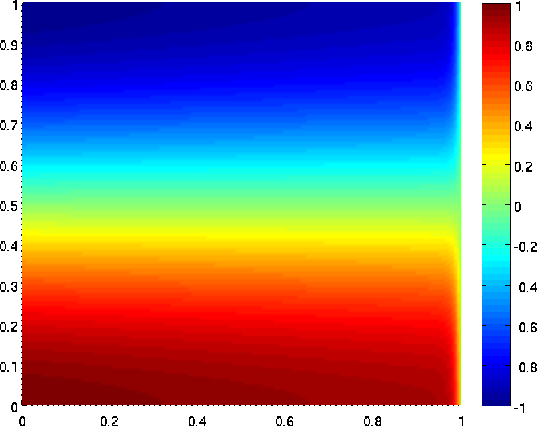
\includegraphics[scale=.37]{figs/wallBC_exact_u.png}
}
\subfigure{
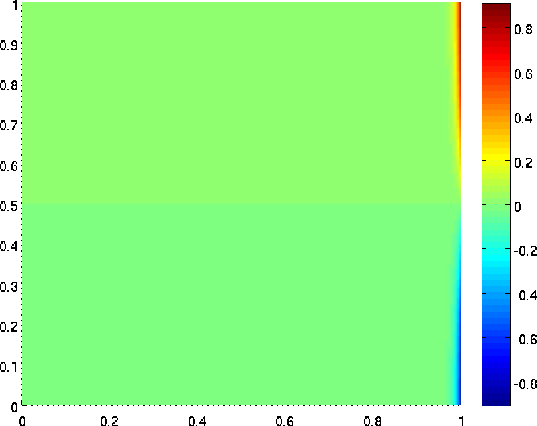
\includegraphics[scale=.37]{figs/wallBC_exact_sigx.png}
}
\subfigure{
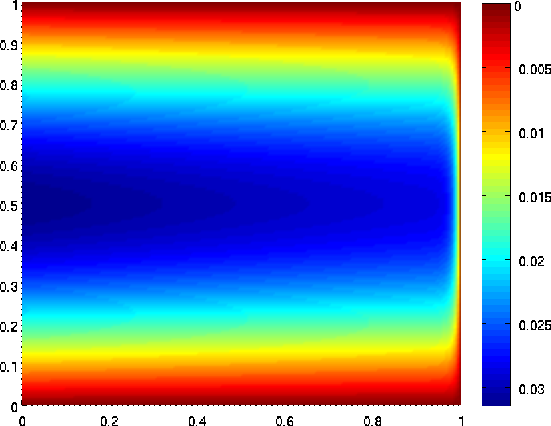
\includegraphics[scale=.37]{figs/wallBC_exact_sigy.png}
}
\caption{Solution for $u$, $\sigma_x$, and $\sigma_y$ for $\epsilon = .01$, $C_1 = 1$, $C_n=0$, $n\neq 1$}
\end{figure}
In each case, we begin with a square 4 by 4 mesh of quadrilateral elements with order $p=3$.  We choose $\Delta p = 5$, though we note that the behavior of DPG is nearly identical for any $\Delta p > 3$.  $h$-refinements are executed using a greedy refinement algorithm, where element energy error $e_K^2$ is computed for all elements $K$, and elements such that $e_K^2 \leq \alpha \max_K e_K^2$ are refined.  We make the arbitrary choice of taking $\alpha = .2$ for each of these experiments.  

\begin{figure}[h!]
\centering
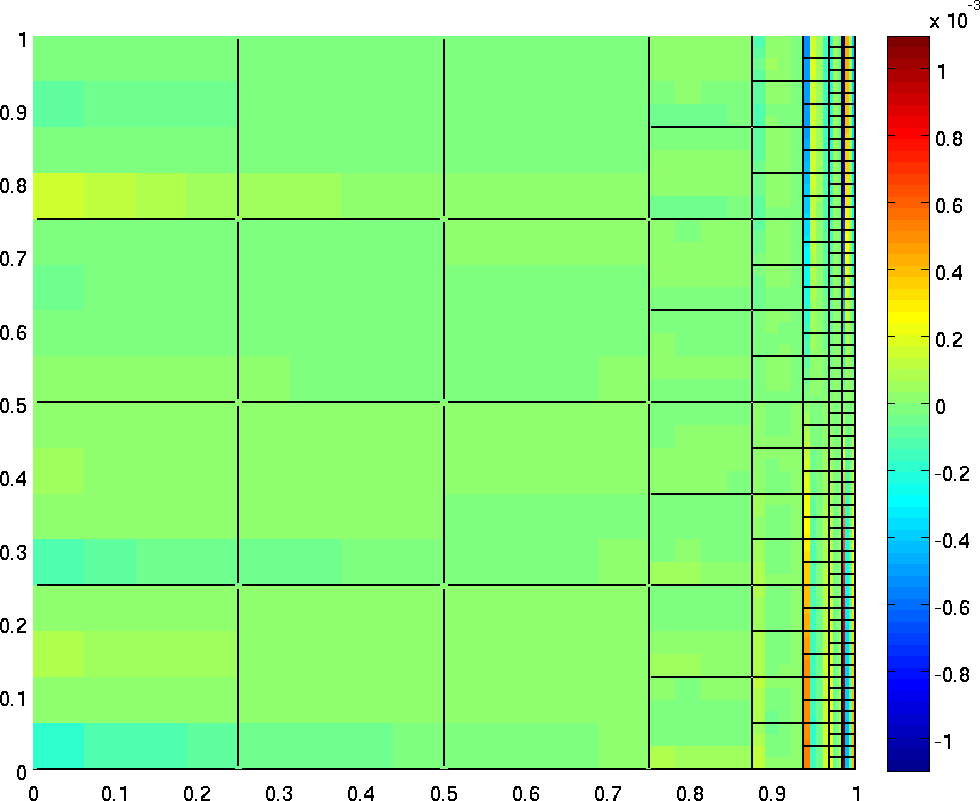
\includegraphics[scale=.4]{figs/u_pointdiff_wallBC.png}
\caption{Adapted mesh and pointwise error for $\epsilon=.01$}
\end{figure}
We are especially interested in the ratio of energy error and total $L^2$ error in both $\sigma$ and $u$.  Stability estimates imply that, using the above test norm, $\|u-u_h\|_{L^2} / \|u-u_h\|_E \leq C$ independent of $\epsilon$.  Figure~\ref{ratios_simple} seems to imply that, at least for this model problem, $C=O(1)$.  Additionally, while we do not have a robust lower bound (i.e.\ $\|u-u_h\|_{L^2} / \|u-u_h\|_E$ can approach $0$ as $\epsilon \rightarrow 0$), our numerical results present a robust lower bound.  

\begin{figure}[h!]
\centering
\subfigure{
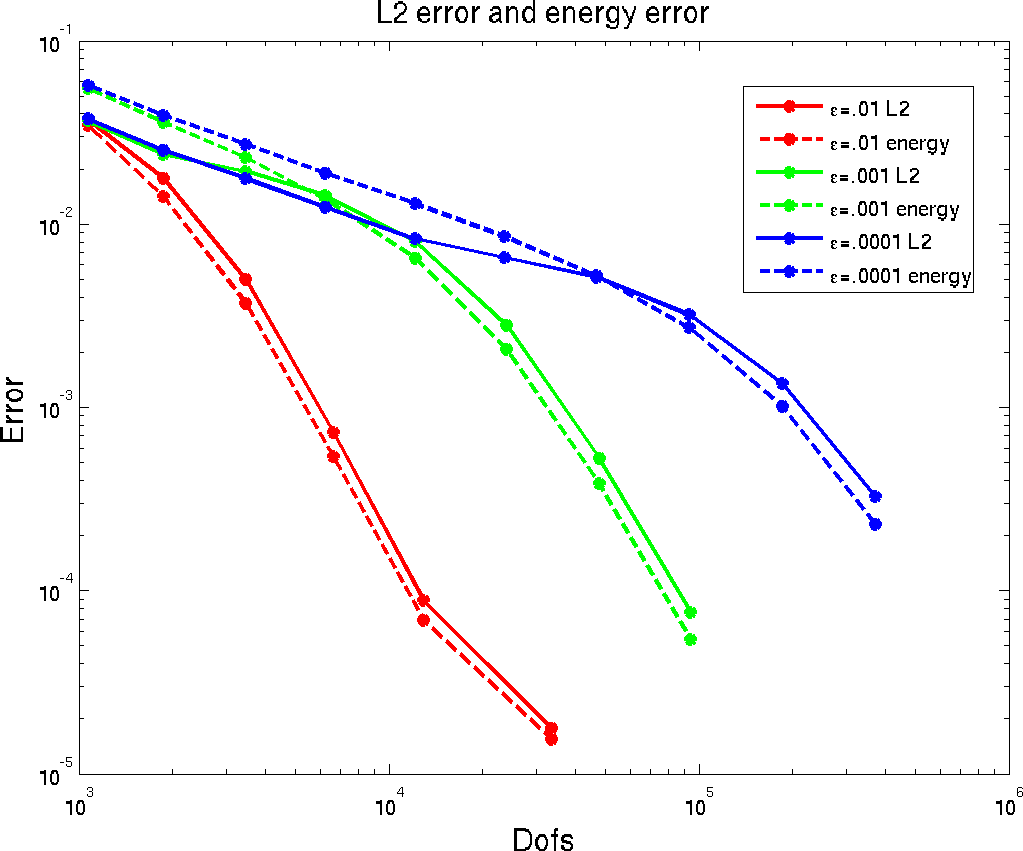
\includegraphics[scale=.38]{figs/errorrates_wallBC.png}
}
\subfigure{
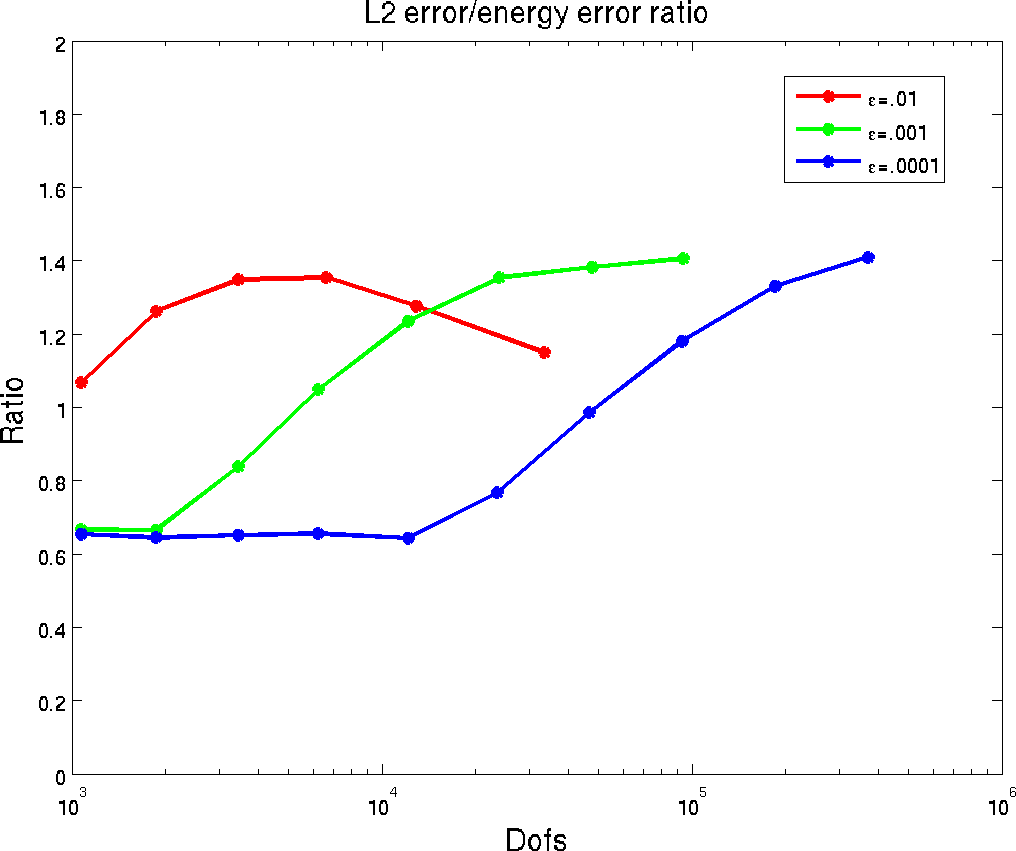
\includegraphics[scale=.38]{figs/L2energyratio_wallBC.png}
}
\caption{$L^2$ and energy errors, and their ratio for $\epsilon=.01$, $\epsilon=.001$, $\epsilon=.0001$}
\label{ratios_simple}
\end{figure}
The effect of a mesh dependent test norm can be seen in the ratios of $L^2$ to energy error; as the mesh is refined, the constants in front of the $L^2$ terms for $v$ and $\tau$ converge to stationary values, and the ratio of $L^2$ to energy error transitions from a smaller to a larger value.  The transition point happens later for smaller $\epsilon$, which we expect, since the transition of the ratio corresponds to the introduction of elements of order $\epsilon$ through mesh refinement. 

We examined smaller $\epsilon$ as well. In \cite{DPGrobustness}, the smallest resolvable $\epsilon$ using only double precision arithmetic was $1e-4$. The solution of optimal test functions is now done using both pivoting and equilibration, improving conditioning. Roundoff effects still appear, but at smaller values of $\epsilon$.

\begin{figure}[h!]
\centering
\subfigure{
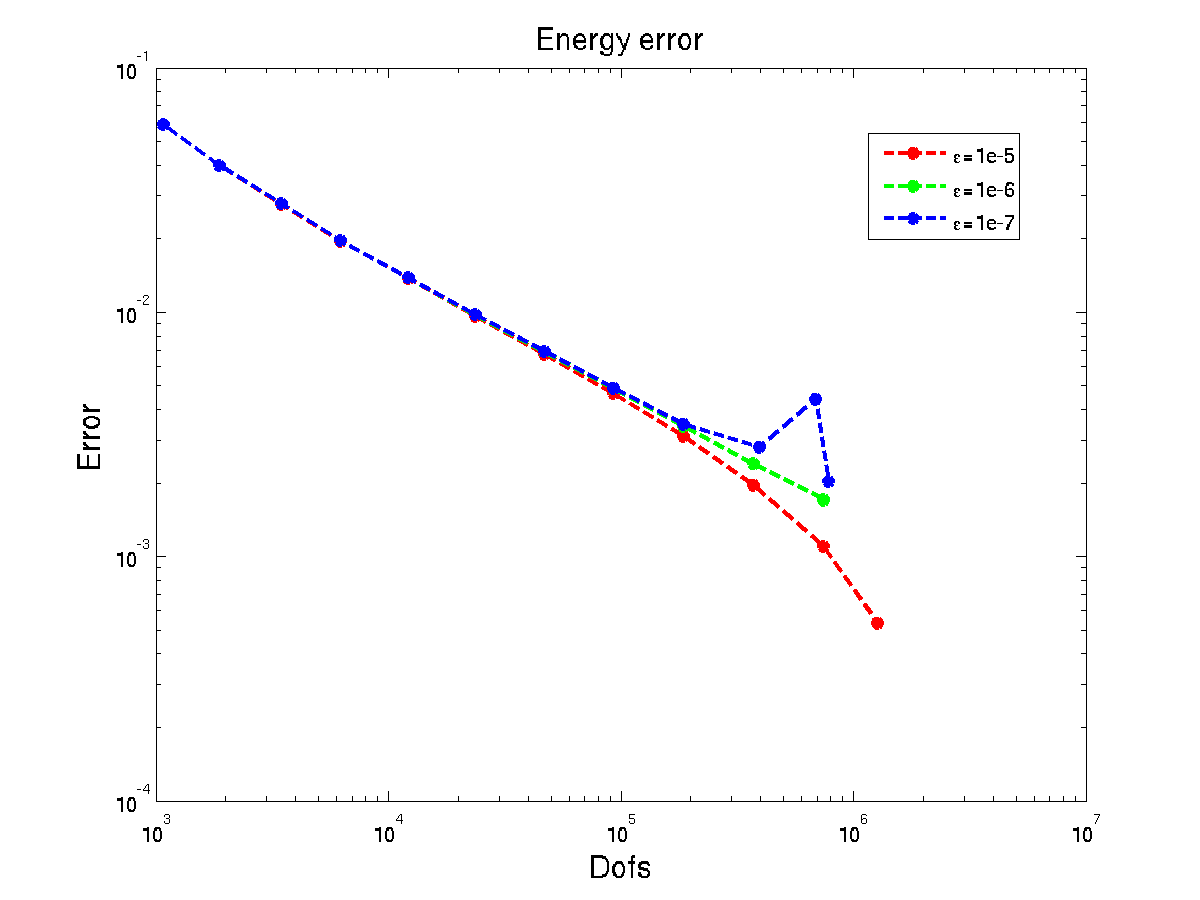
\includegraphics[scale=.38]{figs/roundoff_rates.png}
}
\subfigure{
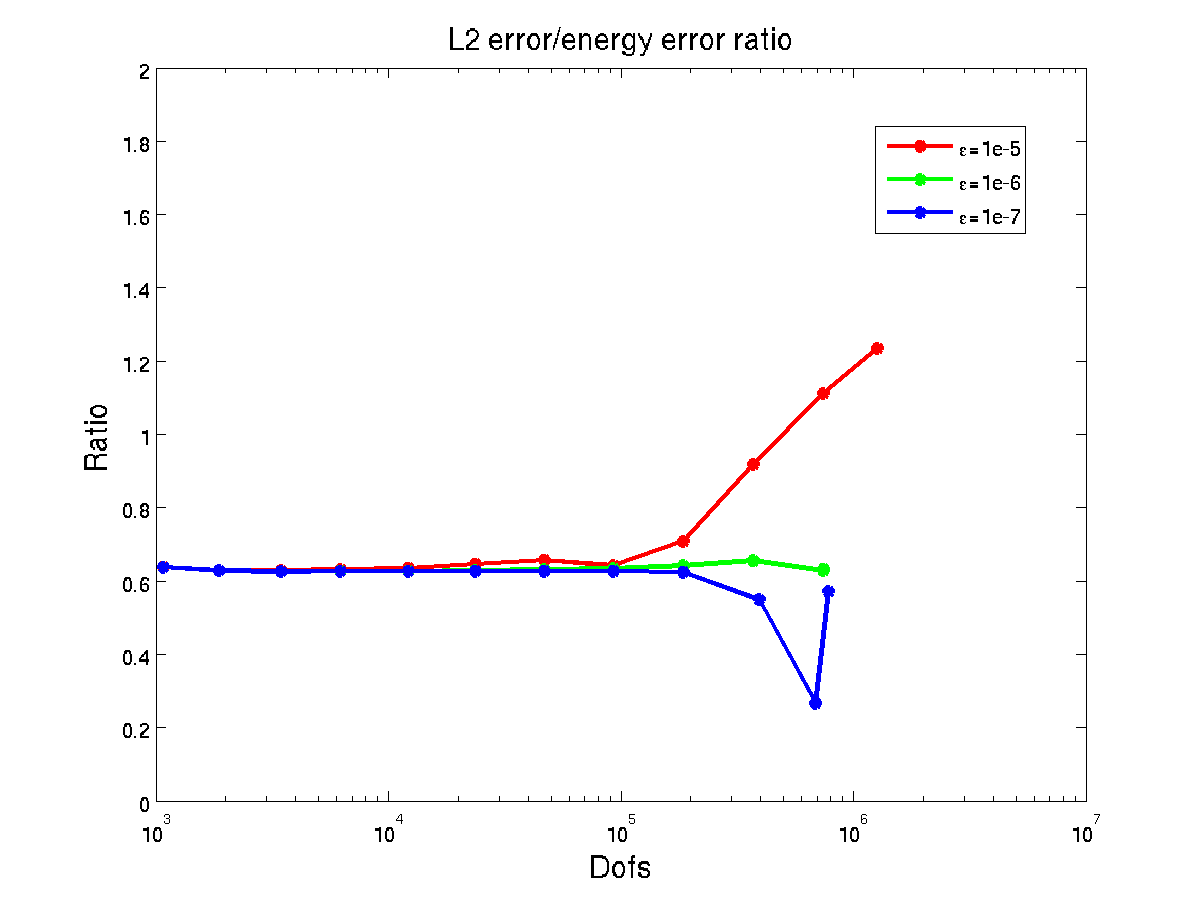
\includegraphics[scale=.38]{figs/roundoff_ratio.png}
}
\caption{Energy error and $L^2$/energy error ratio for $\epsilon=1e-5$, $\epsilon=1e-6$, $\epsilon=1e-7$. Non-monotonic behavior of the energy error indicates conditioning issues and roundoff effects.}
\label{roundoff_figures}
\end{figure}

Without anisotropic refinements, it still becomes computationally difficult to fully resolve the solution for smaller $\epsilon$. Regardless, for all ranges of $\epsilon$, the robustness of DPG remains constant, as indicted by the rates and ratio between $L^2$ and energy error in Figure~\ref{roundoff_figures}. For $\epsilon = 1e-5$, we observe that the ratio of $L^2$ error increases, corresponding to the scaling of the test norm with mesh size (the transition in test norm occurs after 8 refinements, which, for an initial $4\times 4$ mesh, implies a minimum element size of about $1.5e-05$. At this point, rescaled test norm allows us to take advantage of the full magnitude of the $L^2$ term for $\|v\|$ and $\|\tau\|$ implied by our adjoint estimates). By analogy, for smaller $\epsilon = 1e-6, 1e-7$, the transition period should begin near the 10th and 11th refinement iterations; however, we do not observe such behavior. For $\epsilon=1e-6$, the ratio simply remains constant, but for $\epsilon=1e-7$, we observe roundoff effects, as the energy error increases at the 11th refinement. Since DPG is optimal in the energy norm for a fixed test norm\footnote{While the test norm changes with the mesh, it increases monotonically. A strictly stronger test norm implies $\frac{b(u,v)}{\|v\|_1} \geq \frac{b(u,v)}{\|v\|_2}$ for any $\|v\|_1 \leq \|v\|_2$}, we expect monotonic decrease of the energy error with mesh refinement. Non-monotonic behavior indicates either approximation or roundoff error, and as there was no qualitative difference between using $\Delta p = 5$ and $\Delta p = 6$ for these experiments, we expect that the approximation error is negligible and conclude roundoff effects are at play. 

\subsubsection{Neglecting $\sigma_n$}

In practice, we will not have prior knowledge of $\sigma_n$ at the inflow, and will have to set $\beta_n u - \sigma_n = u_0$, ignoring the viscous contribution to the boundary condition.  The hope is that for small $\epsilon$, this omission will be negligible. Figure~\ref{ratios_noSigma} indicates that, between $\epsilon = .005$ and $\epsilon = .001$, the omission of $\sigma_n$ in the boundary condition becomes negligible, and both our error rates and ratios of $L^2$ to energy error become identical to the case where $\sigma_n$ is explicitly accounted for, well within the range of $\epsilon$ of physical interest. For large $\epsilon = .01$, the $L^2$ error stagnates around $1e-3$, or about $7\%$ relative error. 

\begin{figure}[h!]
\centering
\subfigure{
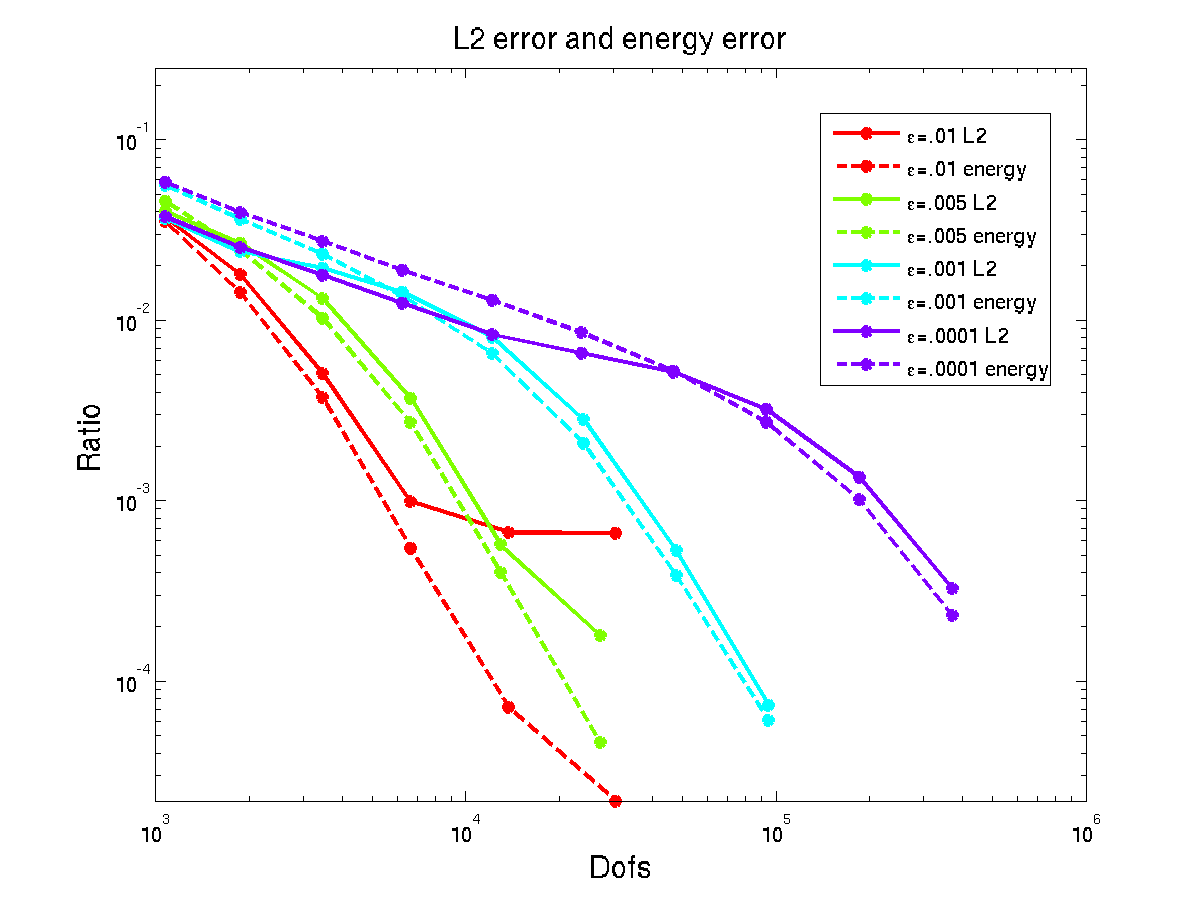
\includegraphics[scale=.38]{figs/rates_noSigma.png}
}
\subfigure{
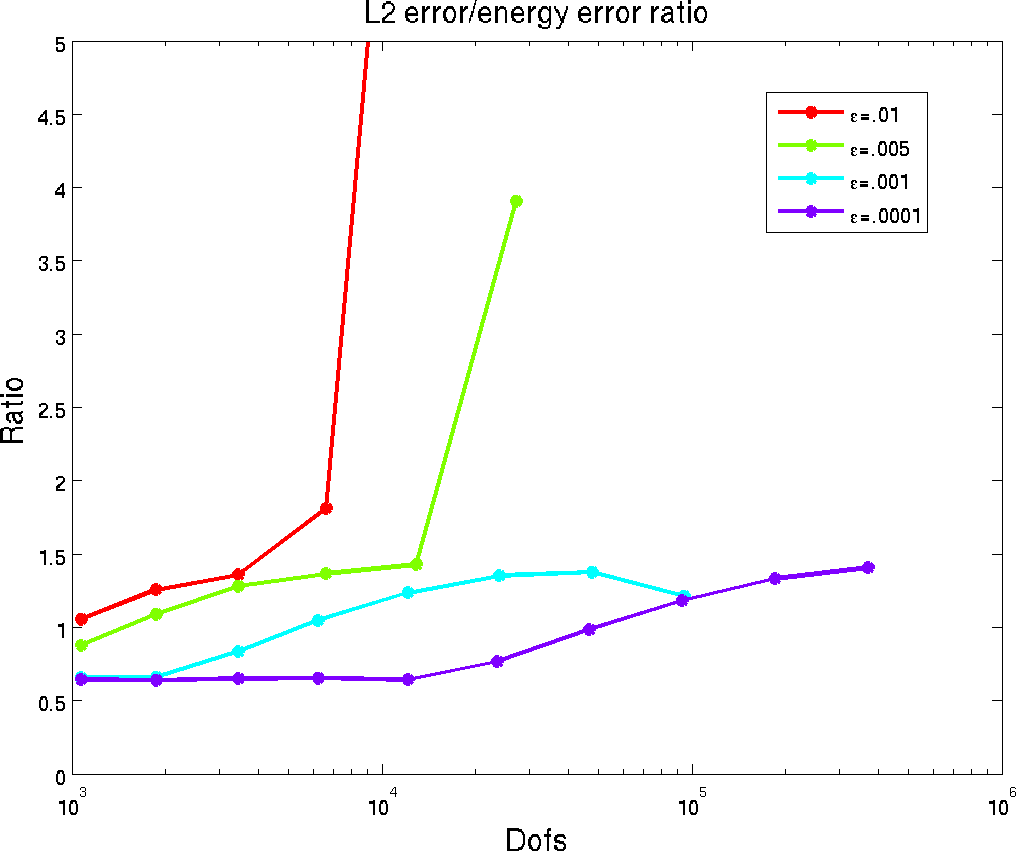
\includegraphics[scale=.38]{figs/ratio_noSigma.png}
}
\caption{$L^2$ and energy errors and their ratio when neglecting $\sigma_n$ at the inflow.}
\label{ratios_noSigma}
\end{figure}

\subsubsection{Discontinuous inflow data}

We note also that an additional advantage of selecting this new boundary condition is a relaxation of regularity requirements; as $\widehat{f}_n \in H^{-1/2}(\Omega)$, strictly discontinuous inflow boundary conditions are no longer ``variational crimes".  We consider the discontinuous inflow condition
\[
u_0(y) = \begin{cases}
(y-1)^2, \quad &y>.5\\
-y^2, \quad &y\leq .5 
\end{cases}
\]
as an example of a more difficult test case. 

\begin{figure}[h!]
\centering
\subfigure{
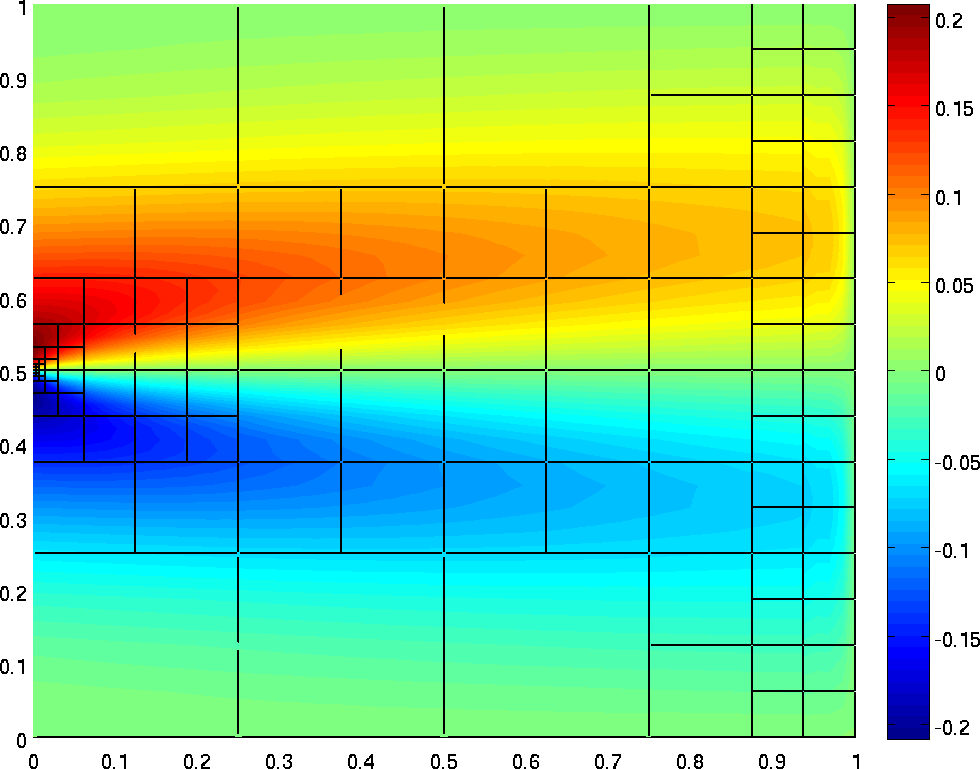
\includegraphics[scale=.38]{figs/disc_hat.png}
}
\subfigure{
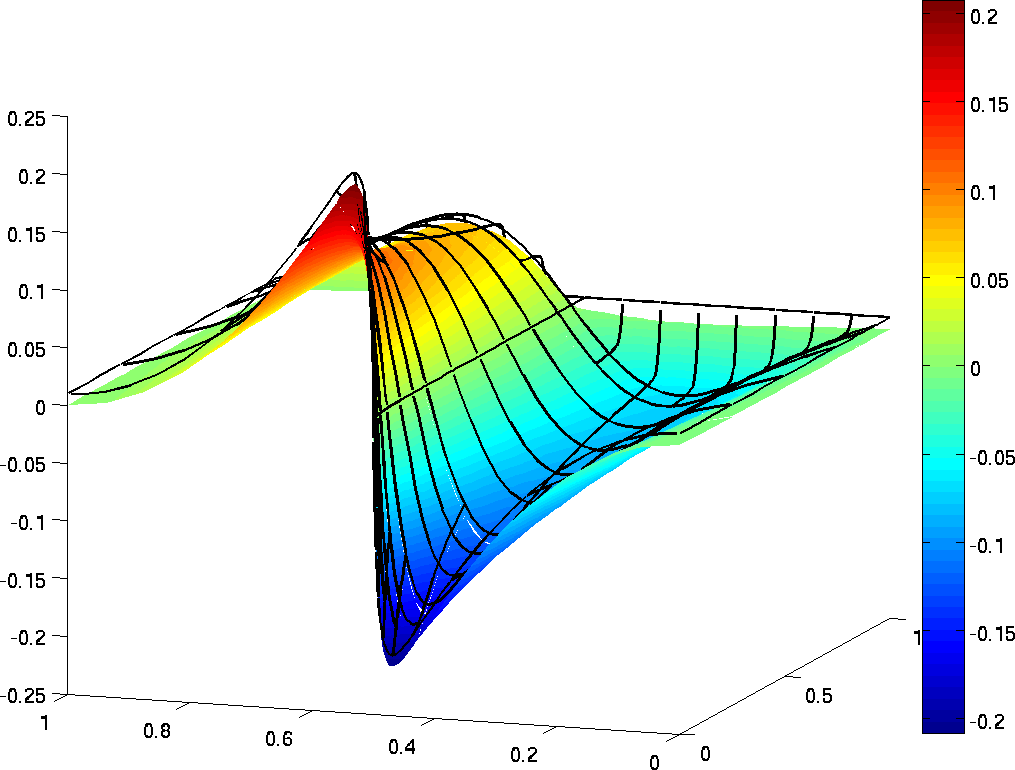
\includegraphics[scale=.38]{figs/disc_hat_surf.png}
}
\caption{Solution variables $u$ and $\widehat{u}$ with discontinuous inflow data $u_0$ for $\epsilon = .01$.}
\label{disc_sol}
\end{figure}
Figure~\ref{disc_sol} shows the solution $u$ and overlaid trace variable $\widehat{u}$, which both demonstrate the regularizing effect of viscosity on the discontinuous boundary condition at $x=0$. In order to compare with an exact solution, we approximate $u_0$ with 20 terms of a Fourier series, giving a near-discontinuity for $u_0$.  

\begin{figure}[h!]
\centering
\subfigure{
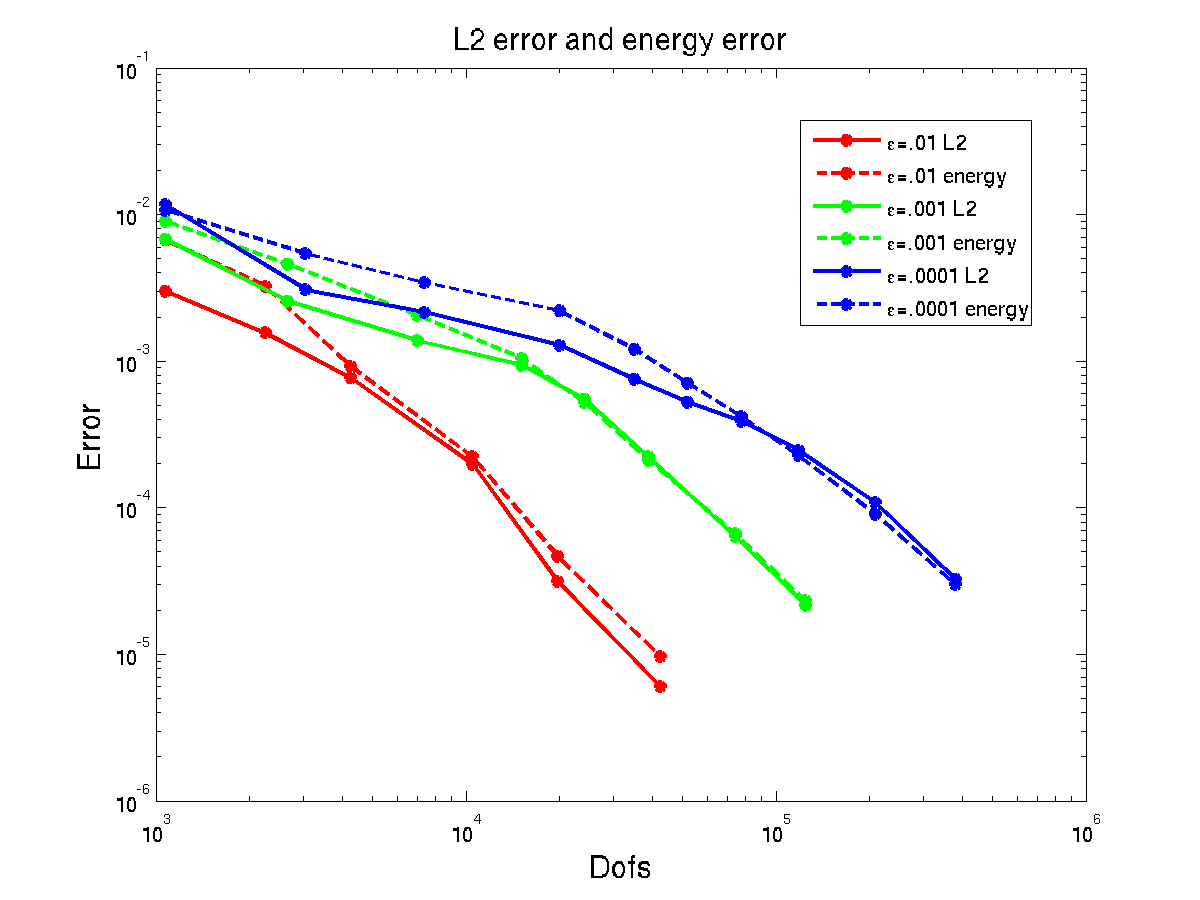
\includegraphics[scale=.38]{figs/rates_disc.png}
}
\subfigure{
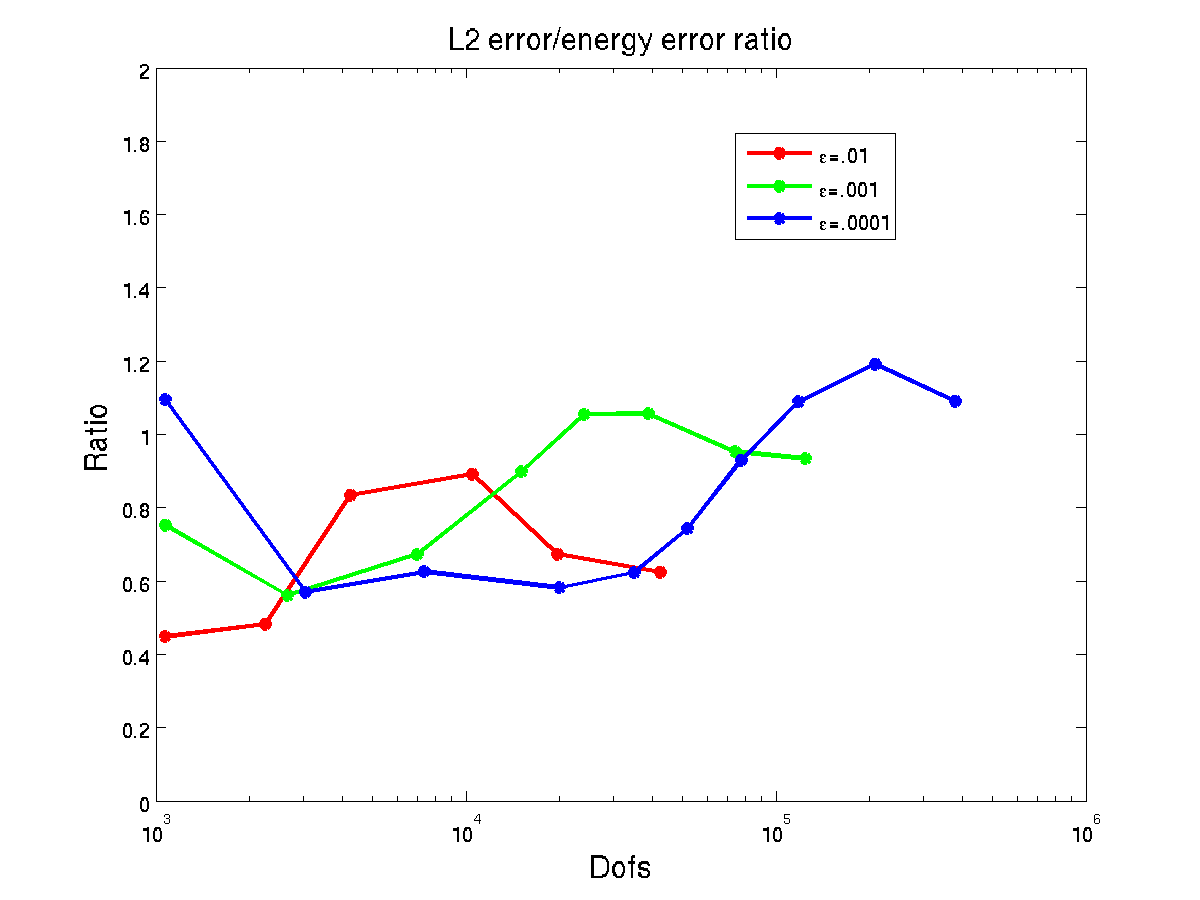
\includegraphics[scale=.38]{figs/ratio_disc.png}
}
\caption{$L^2$ and energy errors, and their ratio for $\epsilon=.01$, $\epsilon=.001$, $\epsilon=.0001$, with discontinuous $u_0$ approximated by a Fourier expansion. }
\label{disc_sol_fourier}
\end{figure}
The ratios of $L^2$ to energy error are now less predictable than for the previous example, due to the ``moving target" nature of the approximation of oscillatory boundary conditions. The numerical experiments were originally performed by applying boundary conditions via interpolation; the result was that the highly oscillatory inflow boundary condition was not sampled enough to be properly resolved, causing the solution to converge to a solution different than the exact solution.  The experiments were repeated using the penalty method to enforce inflow conditions; however, we note that the proper way to do so is to use an $L^2$ projection at the boundary.  When using the penalty method, however, the ratios still remain bounded and close to $1$ for $\epsilon$ varying over two orders of magnitude, as predicted by theory. 

\section{Conclusions}
 
None yet.  Ideas:
\begin{itemize}
\item Explanation of choice of boundary condition and why it impacts stability
\item Interpretation of weight as allowing diffusion to work on the boundary.  
\item Note results have worked for Burgers, and expand on how they would apply to Navier-Stokes
\end{itemize} 
 

\bibliographystyle{plain}
\bibliography{paper}

\end{document}